\documentclass{article}

% Appearance
%--------------------------------------
\usepackage[a4paper,width=170mm,top=18mm,bottom=22mm,includeheadfoot,marginparsep=2cm]{geometry}
\usepackage{url}
\usepackage{enumitem}
%--------------------------------------

% Language
%--------------------------------------
\usepackage[utf8]{inputenc}
\usepackage[T2A]{fontenc}
\usepackage{hyphenat}
\hyphenation{he-lio-trope opos-sum}
\usepackage{csquotes}
%--------------------------------------

% References
%--------------------------------------
\usepackage{biblatex}
\addbibresource{biblio.bib}
%--------------------------------------

% Footnotes
%--------------------------------------
\usepackage[hang]{footmisc}
\setlength{\footnotemargin}{14pt}
\setlength{\skip\footins}{20pt}
%--------------------------------------

% Columns
%--------------------------------------
\usepackage{multicol}
\setlength{\columnsep}{24pt}
%--------------------------------------

% Graphics
%--------------------------------------
\usepackage{graphicx}
\graphicspath{{images/}}
%--------------------------------------

% Tables
%--------------------------------------
\usepackage{array, tabularx, caption, boldline}
\usepackage{graphicx}
\usepackage{cellspace}
\usepackage{makecell}
\renewcommand\theadfont{\normalfont\bfseries}
\def\arraystretch{2}
%--------------------------------------

% Math
%--------------------------------------
\usepackage{amsmath}
%--------------------------------------

\title{\vspace{-3.85em}
\includegraphics[width=0.35\textwidth]{logo.pdf} \\ \vspace{24pt} BANKEX Proof-of-Asset Protocol}
\author{The Smart White Paper, version 0.3.1 beta}
\date{October 19, 2017}

\begin{document}

\maketitle

\begin{abstract}
BANKEX \textit{Proof-of-Asset protocol} (\textit{PoA}) is a standard that enables new generation of assets and contracts called \textit{Decentralized capital markets}. We are building Internet of Assets (\textit{IoA}) on the principles of Bank-as-a-Service (\textit{BaaS}), powered by Internet of Things (\textit{IoT}) and Artificial Intelligence (\textit{AI}) technologies. \textit{PoA} protocol is open for 3rd party fintech providers, AI and IOT labs, traditional financial institutions and asset owners.
\end{abstract}

\vspace{24pt}

\begin{multicols}{2}

\tableofcontents

\section{Introduction}

\subsection{Disclaimer}

You are reading The Smart White Paper.

It was developed by the BANKEX team and describes a decentralized technology for control of liquidity of smart assets based on the Proof-of-Asset Protocol.
	
We provide the description of the technology, based on our level of knowledge and development. We hope you will find it valuable. However, there are certain commitments we are unable to make in regards to the technology of the protocol.  
Neither BANKEX, nor its suppliers and distributors provide any guarantees regarding the Proof-of-Asset Protocol software, aside from those mentioned in the provided and additional Terms of Use. We take no responsibility in regards to the contents of the protocol software, its special functional capabilities, availability and compliance with your requirements. All services are provided \enquote{as is}.

Local law of certain countries ensures guarantees such as vendibility, serviceability in certain fields, investor protection and intellectual property rights protection. Aside from situations outlined in the legal system, we exclude any and all implied warranties.

After reading The Smart White Paper you may decide to take part in the development of new decentralized technologies, using your knowledge, time and financial resources. Therefore by reading this text, you assume the unconditional obligation that, in the event of being a citizen of USA, China, Singapore, Russia or any other country, any lawsuit with any claimant, where your name is featured as an involved party, we receive a guaranteed right to charge you as a private party for the full amount of losses, including any fines or legal costs, including in the event of your using software (VPN, Class Action, etc) to conceal your true country of residence. 

\subsection{BANKEX Proof-of-Asset Protocol}

BANKEX is an organization that unites members of the financial markets in order to build a community and implement the Proof-of-Asset Protocol enables community members to profit from mutual use of assets. 

The product of BANKEX is the Proof-of-Asset Protocol, which solves the issue of non-fungible asset liquidity. Proof-of-Asset means the token released as part of the protocol is ensured with an asset. 
The know-how of BANKEX is the Proof-of-Asset protocol, in essence a combination of BaaS (Bank-as-a-Service) and blockchain technologies. We take a client asset, primarily on the financial market, we tokenize it, then, without waiting for the portfolio to accumulate critical mass, we turn this asset into money for the bank.  This is made possible through formation of a single pool of similar assets (e.g., pool of banks) thereby creating a marketplace, where banks benefit from liquidity and investors benefit from a predictable and transparent cash flow.

\subsection{Specification of Examples in White Paper}

All examples and demonstrations in this White Paper are used only as demonstrative examples of the SmartDeal technology. The business of BANKEX involves manufacturing fintech products and tokenizing primarily financial assets, although we do not think it impossible to apply the Proof-of-Asset Protocol in other fields, with approval from the BANKEX Foundation in case of non-financial Smart Assets. In our case, first and foremost we create liquidity for financial assets.

\subsection{Game Theory Behind the Proof-of-Asset Protocol}

Game Theory\footnote{\textbf{Game theory} is the study of the ways in which \textit{interacting choices} of \textit{economic agents} produce outcomes with respect to the \textit{preferences} (or \textit{utilities}) of those agents, where the outcomes in question might have been intended by none of the agents \cite{stanfordGameTheory}.} is a branch of mathematical economics focusing on the outcomes of conflicts between players, and the optimality of their strategies.

Game theory is one of the prime fundamental directions in economics. 11 scientists specializing in game theory have received the Nobel Memorial Prize in Economic Sciences, including John Nash \cite{nash1950}, \cite{nash1951}, responsible for introducing one of the key concepts in game theory, known as the Nash equilibrium. It is a state in which a single player cannot benefit by changing strategy while the other players keep their set of chosen strategies unchanged. 

Analysis carried out according to game theory indicates that the global financial market is currently trapped in the sub-optimal equilibrium of the prisoner’s dilemma. This dilemma is a fundamental problem of game theory, illustrating how players will sometimes fail to cooperate even if it was in their best interest.

We see that players in financial markets distrust each other and keep overpaying for an inefficient set of various ratings, scores and audits, although these are frequently wrong (as with the Enron scandal and the subprime mortgage crisis). This inefficiency leads to high costs and often losses, which in turn raise the cost of capital and lead to a lack of access to capital for decentralized small businesses or borrowers. Another issue derived from this dilemma is the obstructing cost of deployment to the public market. If this barrier is removed, then the market itself is cable to evaluate every asset based on the collective wisdom of all trading participants, as the increase in volume of transparent and authentic trade operations provides more information that can be used by the market to verify the assets.

We offer a solution~--- the Proof-of-Asset Protocol, the point of which is an instant audit of the asset. Now every investor is aware of the status of his investments in non-public companies and assets. Equipped with this tool, the market will force certain businesses to change (lawyers, accounting, auditors, and in separate cases banks and collectors). What is our plan? We will begin by modernizing the mechanisms of assigning and validating ratings, as the cash flow recorded on the blockchain using the Proof-of-Asset protocol is transparent, understandable, as well as much faster and cheaper. In essence, the asset’s state is being constantly monitored by the logic of smart-contracts.

In turn, the increased amount of information on economical operations and their authenticity grant new opportunities for the development of an economical AI, building sufficiently precise artificial intelligence systems for risk evaluation, making the cost of such calculations approach zero. This would enable the creation of a competitive market of economical AI working for the good of modern society. 

\section{Modern Financial Markets}

\subsection{Bank-as-a-Service (\textit{BaaS}) Business Model}

Bank-as-a-Service (\textit{BaaS}) is a business model that makes it possible to build new financial products that are integrated with multiple existing technological solutions and jurisdictions. 

On one side of these platforms are originators in various jurisdictions with various technologies, and on the other are fintech-companies wishing to launch a new product or expand to a new market. Thanks to the platform, they are able to do this quickly and efficiently, without the need to work out integration with the legislation of every country and every new bank from scratch. Since the platform already contains technological and legal integration, it can provide access to a new player more cheaply and more quickly. 

\textbf{The originator in the BaaS model} is a storefront, essentially establishing access to the end client, be it a bank, a fintech company, an internet platform, a stock exchange or an insurer. It is critical that when building the BaaS business model, the originator of the platform maintains his client and access to the client under his control, but at the same time he provides the client with the most up-to-date and competitive products on the market by the best tech (fintech, IT) companies on the market. It’s an excellent solution to preserve and monetize clients.

How does an end client see it? Like a bank~--- he does not have to see the third party provider.

There exist several levels of integration of participants of the BaaS model: from primitive analogue integration, where an employee would have to re-enter data into a separate service, to fully automated integration. The originator makes the choice of whichever model of work with an end client is most beneficial to him, either where the end client is shown that the company he is interacting with provides services by outside service providers, or where the end client sees the entire product line under the originator’s brand.

Some researchers call this conception \enquote{The Lego Bank} which owns no pieces but assembles the pieces into different form factors.  The constituent pieces are all the same.  It is how you put the pieces together that makes the difference.  Like Lego, you can build the pieces into a Castle, a House or a Winnebago.  It’s all about how you click pieces together \cite{skinner2017baas}.

As a result, the Bank-as-a-Service platform is a unified window, where corporate or retail clients can choose and receive services that are being offered by various banks and tech companies in various countries. This platform takes over technical and legal integration of various players on the financial market.

\subsection{Decentralized BaaS Model}

According to McKinsey \& Co., there are three main trends in banking evolution:

\begin{itemize}
\item automation;
\item increased regulation;
\item increased pace of technological development.
\end{itemize}

Blockchain allows to automate different processes and banks can benefit from it a lot. Accounting, legal and risk parts might be automated. McKinsey \& Co. states that blockchain, based on advanced cryptography, might allow doing such operations in the most effective, safe and transparent way in human history.

\textbf{For global players, adaptation to such trends will become a vital issue}. Enhanced financial regulation will force participants  to use partner BaaS platforms as adaptation to new jurisdictions independently will become prohibitively expensive. Fast tech development,  which many of the banks can’t handle, will drive banks interest in using other fintech companies’ services. It will drive a demand for BaaS usage.

\textbf{Decentralized BaaS is the future of banking. Why?} The world has changed and financial streams are becoming global. They are no longer easily controlled by common tools. Regulators and central banks, defining the movement of the market, are responding to this with more strict regulations. In turn, banks respond by creating as many service offerings as permitted by their license beyond their confines. They aim to create innovative services, leaving only themselves with just the core.

This trend creates the risk of a bank evolving into something more similar to a telecommunication company~--- a company with a license that no longer sees its clients.

At BANKEX we see this risk, but believe it is right for banks to preserve the status of the most important key element of the world’s financial ecosystem. Fintech and IT companies should not be disrupters of the banking system. Instead they should supplement each other in a mutually beneficial way.

Several years ago, banks and innovative technologies existed separately, with banks expressing an interest in external IT products such as certain separate features. Today the market has changed, leading banks of the world work more and more closely with fintech companies, while the fintech companies in turn ceased to see themselves as disruptors triumphing over banks and instead view themselves as partners to banks. Everyone acknowledges that offline bank departments will remain, even if nobody goes to them, as foundations of faith in the system. A customer must understand that the financial service he receives is that of a bank, the bank actually exists, it has a department in the city, to which the customer can go in case of an issue for assistance. This reason at least will remain. This isn’t just a domain that might close tomorrow and leave its end client alone with their issue. On the other hand, fintech and blockchain companies acknowledge that the market share occupied by their products is too small, below 10\%, and in order to amplify it, they must partner with banks.

In other words, fintech products must end up at banks. Clients, in turn, will purchase and use innovative financial products much more willingly if they can do so under the brand of a familiar bank. It’s worth noting that some banks will remain skeptical about integration with fintech companies. Luckily, the banking community understands that fighting innovation will only result in market share loss.

On the other hand, FinTech innovation alone is not sufficient to absorb the exorbitant transaction flows and and vast financial streams. One explanation is that banks don’t trust one another and they don’t trust technological companies. They are afraid of losing their client-base by partnering with a stronger or more technologically advanced player. They are concerned that upon close examination their products will not be competitive compared to alternatives. They are afraid regulators would penalize them for use of innovations in their base products. Another important note is that decisions regarding such risks are made by top-managers, most of whom are more concerned with protecting their reputation than introducing innovation.

Technological progress has presented us with solutions to such issues~--- organizing mutual trust of participants in the system and trust in operations in the system based on decentralized data storage and automated smart-contracts.

Many professional market players admit that a decentralized BaaS business-model is an optimal path to collaboration between classic banks and financial companies with cutting edge IT companies and continually growing decentralized technological companies of the future.

Front service of clients remains in the hands of the banks, while products are presented by narrowly-oriented product banks or companies. 

We believe that the \textit{B2B2C} combination of business-models and technologies is the key to BANKEX’s success.

\subsection{Classical Microservice Architecture}

Microservice architecture is a network of module services that can be deployed independently from one another.

Microservice architecture is an approach to structuring applications whereby they are broken down into smaller independent internal components.

\paragraph{Advantages of Microservice Architecture:}

\begin{itemize}
\item autonomous ownership for different microservices within an application;
\item agility, application micro-components can be developed and tested in autonomous decentralized teams much faster;
\item improved scalability (scaling independent of other components, on-demand scaling);
\item continuous delivery and deployment of micro-components.
\end{itemize}

A monolithic architecture is much easier in implementation, control and deployment, while microservices require careful management, as they are deployed on different servers and use API.

Such architecture allows technically complicated applications to constantly evolve without the need to wait for the release of a new version of the product to make changes. There is no need to release an updated version of the product, if the changes apply only to a small part of the product. That’s why it’s possible to customize for various business tasks of every enterprise, department or person.

Notably, microservices can be fully managed by different teams in compliance with different standards and are also more available: even if one of them crashes, it does not lead to the crash of the entire application. A unified architecture facilitates work in situations where multiple modules need to interact with one another, or where classes need to be transferred from one module to another. At the same time microservices can guarantee that there will be no shared states between the modules. Finally, microservices allow you to use multiple technologies and languages, depending on business needs (Figure~\ref{fig:microservice-vs-monolyth}).

\begin{figure*}
  \centering
  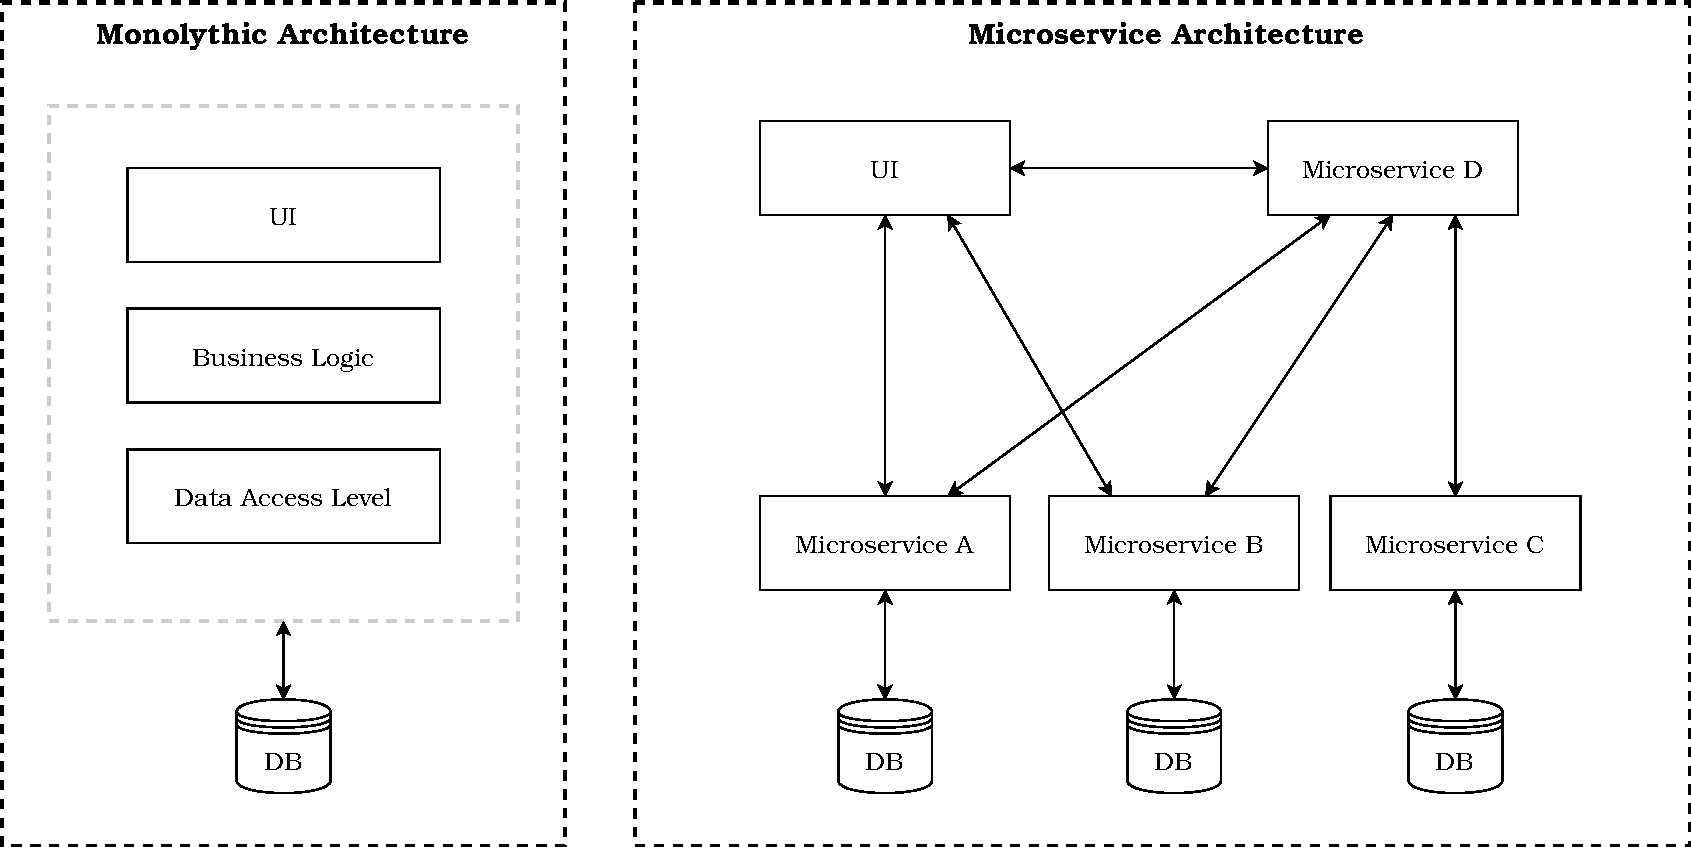
\includegraphics[width=\textwidth]{microservice-vs-monolyth.pdf}
  \caption{Monolythic vs. Microservice Architecture}
  \label{fig:microservice-vs-monolyth}
\end{figure*}

\subsection{Blockchain Serviсe Architecture}

On an Ethereum blockchain micro-service, architecture is used in the implementation of external oracles. At the same time, the Ethereum network is itself an example of network that uses the concept of micro-services, since it contains all the characteristic features of micro-services
(Figure~\ref{fig:blockchain-microservice-architecture}):

\begin{itemize}
\item excess and reservation, as each node of the network is autonomous;
\item service discovery for automatic configuration of network topology;
\item extensibility through the use of other types of micro-services (such as oracles, micro-services allowing to display statistics, etc.).
\end{itemize}

\begin{figure*}
  \centering
  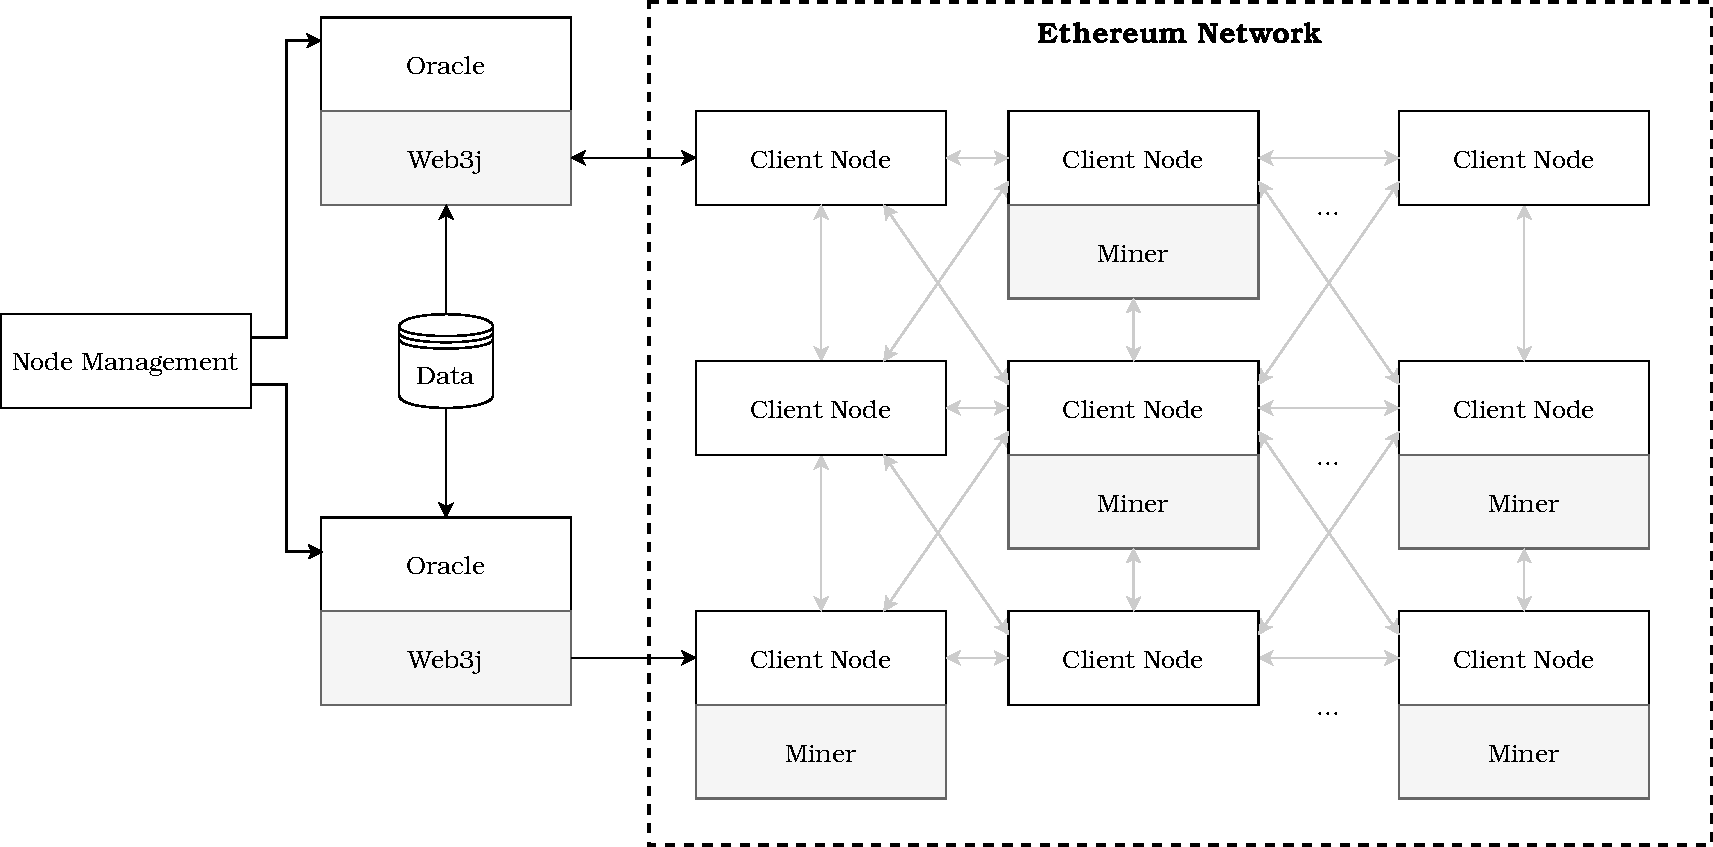
\includegraphics[width=\textwidth]{blockchain-microservice-architecture.pdf}
  \caption{Blockchain Microservice Architecture}
  \label{fig:blockchain-microservice-architecture}
\end{figure*}

The logic of the BANKEX liquidity protocol is based on the concept of the Ethereum smart contract\footnote{The phrase \enquote{\textit{smart contract}} was coined by Nick Szabo initially in \cite{szabo1996} and later in \cite{szabo1997}.}, and accordingly uses all of its infrastructure advantages. At the same time, technically, the BANKEX protocol is a series of smart contract updates, however these smart contract updates are not micro-services themselves, the micro-services are in relation between API calls themselves. From our side, the business tasks of the protocol, which require a classical micro-service architecture, are realized through the creation of the oracle system. Protocol oracles are designed strictly according to the principles of the micro-services, that is, the instances of these oracles should be automatically added under the required conditions. In this case, dynamic balancing of the number of oracle instances is used. Part of the BANKEX oracles is implemented on the basis of Microsoft Azure cloud technologies, since it's one of the most bank friendly platforms. An example of the protocol logic was realized through the interaction with the signals from Internet of Things sensors.

But for the description of the BANKEX Proof-of-Asset protocol the definition of the micro-service architecture is not entirely correct. BANKEX team calls it the \textit{Blockchain Service Architecture}.

\paragraph*{Blockchain Service Architecture} is a sequence of smart contracts, every step of which can be customized by a predetermined pool of actors validated for the particular step of the included smart contracts, while the contents of contracts in a step and the number of steps are embedded in the business logic necessary to tokenize the Smart Asset.

It is an asset tokenization constructor, but one that only works in a sequence of smart contracts correctly arranged after one another, supplemented with oracles connected as micro-services. 

This allows to tokenize an asset with maximum precision and transparency for all participants of the market, while also working in line with the open source BANKEX Proof-Of-Asset protocol. 

\subsection{Complexity regulation of the Blockchain Service Architecture}

We often hear from technical experts: Your protocol is too complicated. Other technical gurus say~--- your protocol is too simple. Yes, they are correct. The complexity of the BANKEX protocol, which is based on the Blockchain Service Architecture, is regulated by the increase/decrease in the number of smart contracts in the tokenization logic (Figure~\ref{fig:smart-asset-contract-chain}).

\begin{figure*}
  \centering
  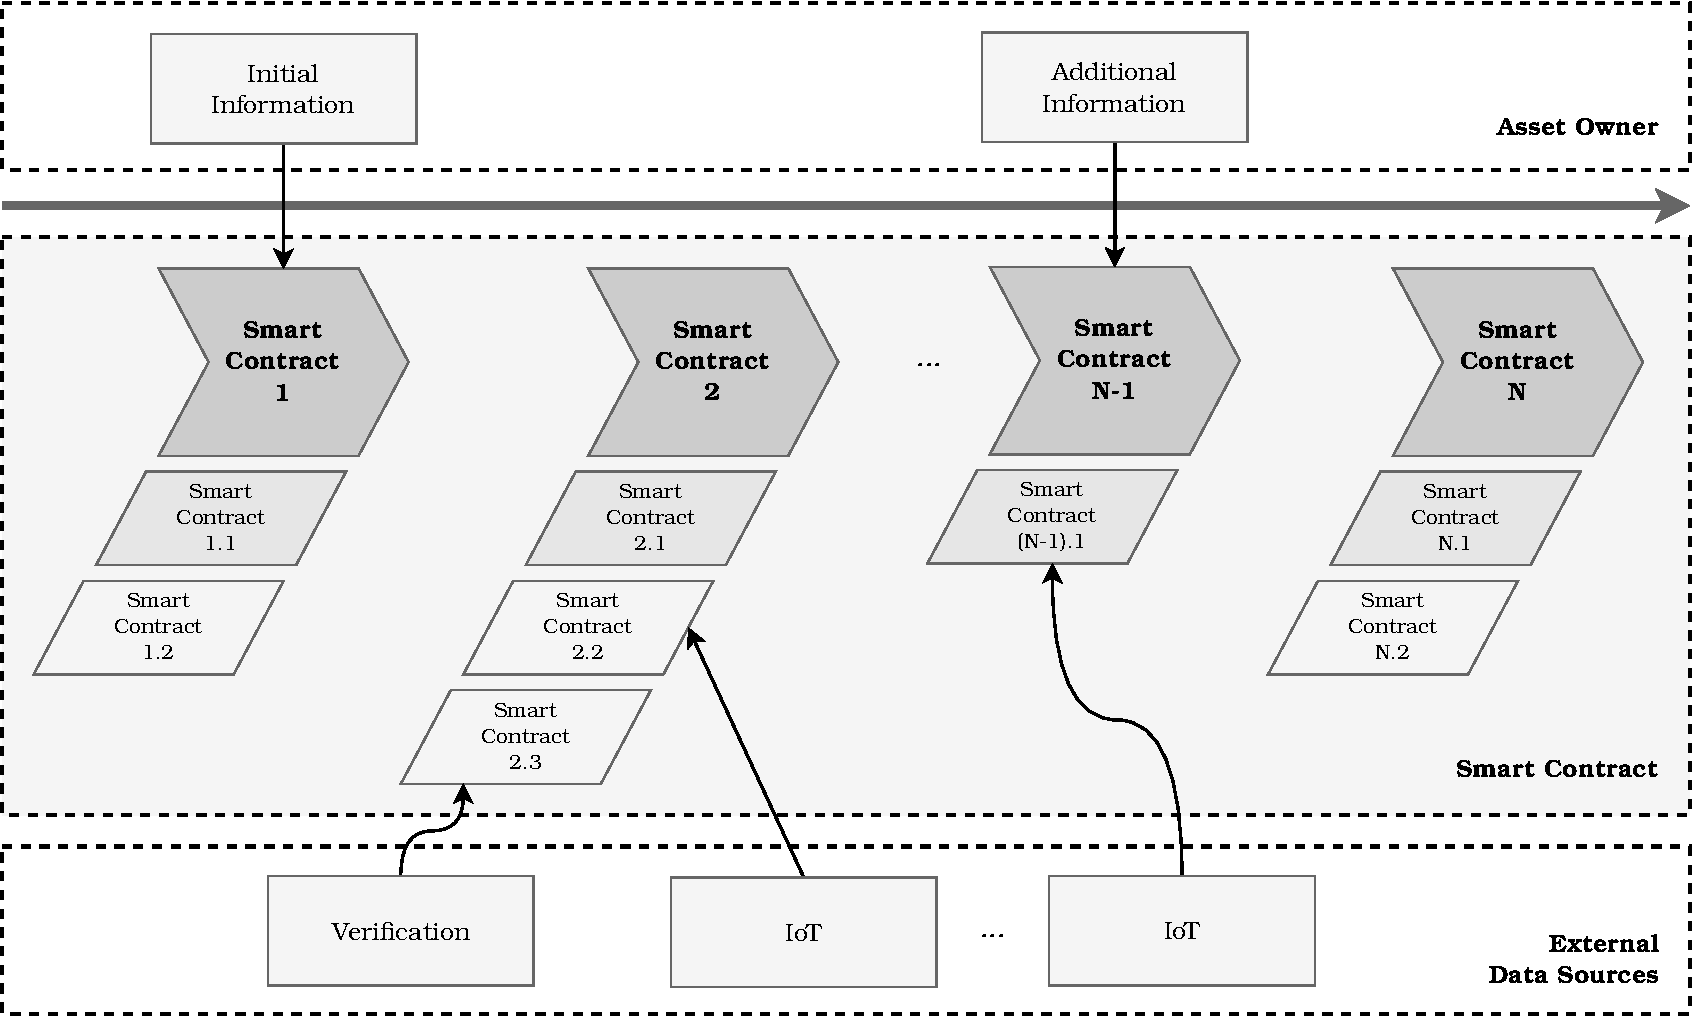
\includegraphics[width=\textwidth]{smart-asset-contract-chain.pdf}
  \caption{Blockchain~SA Smart Contract Chain}
  \label{fig:smart-asset-contract-chain}
\end{figure*}

The creation of a smart asset of a certain type does not necessary use all the steps that are laid out in the Blockchain Service Architecture, only the steps of the smart contract chain that are required by a particular Smart Asset are used. The simplest Smart Asset consists of three steps: initialization, validation, and valuation. And in this case the Smart Asset will fulfill its mission~--- make the asset liquid. It’s not complicated at all. 

At the same time, BANKEX is an old company in the sphere of financial technologies, classic fintech. We know very well how complex financial tools can be, and how difficult it is to properly formalize them. Our solution is the Blockchain Service Architecture~--- exactly what you need. You can add any level of complexity to the asset tokenization chain which will result in a Smart Asset.

Moreover, the Smart Asset retains all the features of a blockchain Smart Contract~--- everyone is able to see what value is behind it and how truthful it is. 

You can add your own logic block to the BlockchainService chain~--- Proof-of-Asset Protocol, because it is an open source code. To do that~--- you will need to address the BANKEX Foundation community.

\subsection{Benefits of the Blockchain Service Architecture}

\paragraph*{Why would the service architecture of the future use blockchain?} In the existing infrastructure, a large application or product consists of a large number of modules which are almost always developed by different teams, and, even if the teams work within the same bank, they still requires a large number of cash flows between different participants in the system and a large amount of agreements and inspections. It is costly, time consuming, and very likely to result in mistakes, including system errors.

Blockchain helps automate the chain of transactions, increasing reliability, transaction transparency and removing inefficiencies and bureaucratic hurdles. It lowers the risk of human mistakes and for many operations completely removes the need for human intervention. This will make your business faster, lower your costs and increase the market's trust in you.

Finally, Blockchain Service Architecture will allow you to build, in the best way, a product line fitting with the trend of personalization and to offer unique solutions to consumers exactly when they really need it.

Blockchain technologies are perfectly suited for this task, as they provide an infrastructure with an open register of immutable operations. The first release of the Proof-of- Asset protocol relies on the established technology of open blockchains, most importantly Ethereum. Technologies for the creation of private blockchains are currently on their way to becoming established and accepted by the industry. Thus the first release focuses on the tokenization of open assets. In the future, the algorithm will be adapted to private blockchains in line with their readiness for industrial application.

We see the current issues with financial instruments from within; we see how many inefficiencies exist between market participants. Our mission is to provide technologies that market participants will like, that will improve upon the current market structure, and that will enable the same people~--- the same market participants, to interact more efficiently and, above all, more profitably.

\subsection{Liquidity Theory in the Context of Tokenization}

Liquidity of an asset is the ability to sell or buy the asset quickly without significant change in its price. Higher liquidity alleviates the trade-off between the price of an asset it can be sold/bought for and the speed of its sale. People have preference for liquidity, such a theory was first introduced by John Maynard Keynes \cite{keynes2017}. Many theories and empirical studies suggest that lower liquidity results in underrated value stored in assets \cite{amihud2005}. 

Making these assets more liquid will help unlock the value.

Protocol of liquidity is a derivative of what we refer to as The BANKEX Proof-of-Asset protocol. We call it that because today, unless it possesses a certain description of characteristics, it is fairly difficult to sell an asset, even if at first glance it appears liquid. For instance, a new consumer good, as an asset, is fully liquid~--- all one needs to do is list it in an online store,  making it possible for an end client to buy it. But not all types of assets and even not all of the simplest consumer goods have deliberately truthful characteristics and a capacity for digitization. The most common example, a used consumer good, requires at least a description of changes to its base characteristics, and then the buyer needs to be convinced that the description of the good is truthful. This, as a result, requires the buyer to check the described characteristics in order to make a purchasing decision. This happens because this “asset” is not digitized at the outset, so the mechanics of selling it become more complicated, compared to the sale of a similar new asset. 

To address this problem, various niche technological services emerged that assist in making an asset more liquid, while also facilitating trust between each sides of the deal. Services do this in different ways, from simple announcement boards, to complex internet-services with risk insurance included. These services make an asset “understandable” to the market, after which said asset becomes significantly more liquid than it initially is.

This is an example of digitization of an asset giving it liquidity.

But tokenization is different from digitization: digitization is about creating descriptions, its consumer characteristics, photographing etc. Tokenization, beyond the aforementioned steps, adds financial components~--- automated smart contracts for deal execution, commands for automatic transactions, formulas for calculation of the asset price, automatic validation of the initial data and much more.

So, digitization is about asset description and its publishing on the market. Tokenization is about asset description, validation by oracles, asset price calculation, automated audit, calculation of cash flows based on its price, execution of the SmartDeal.

One of the major reasons for tokenization of an asset is the possibility to avoid fraud that may be present in the case of classic digitization. A good can be digitized but might also contain false information in its description. Often it is difficult for an asset owner to see the real information about cash flows even if there is no intention to hide them. BANKEX Proof-of-Asset Protocol provides the proof that an asset and its cash flows are authentic.

We remind you that this BANKEX White Paper uses examples and demonstrations only as demonstrative examples of the SmartDeal technology. The business of BANKEX involves manufacturing fintech products and tokenizing primarily financial assets, although we do not think it impossible to apply the Proof-of-Asset Protocol in other fields, with approval from the BANKEX Foundation in case of non-financial Smart Assets. 

\subsection{Mathematical Market Making Models for Smart Asset}

\subsubsection*{What is market making?}

Market maker is a player on a market for a good or security who provides both buy and sell opportunities for traders, thus making this market more liquid. Market makers hold both the security/good and cash in inventories in order to be able to take the opposite side of trading order volume to fix imbalance in buy and sell orders. Market-makers earn on bid-ask spreads, but bear the risks of price decline of their inventories.
 
\paragraph*{Key players:}

\begin{itemize}
\item traders: responsible for creation of purchasing/sell orders;
\item market makers (specialists): display public buy \& sell quotations for a guaranteed number of securities/goods to traders and fulfill orders from traders at these quotations;
\item dealers: buy and sell securities/goods from traders but do not disclose quotes publicly;
\item brokers: carry out orders on behalf of their clients.
\end{itemize}
 
Liquid trade is of great importance for the stability and effectiveness of financial markets. 
 
Market making is an established trading practice, which has inspired much research, both theoretical and empirical. Most of the theoretical research papers model market maker as a single player with whom other market players can trade, with no trading activity apart from that. On the other hand, there are some research papers where market makers compete with middlemen (dealers/brokers). In this model, the author introduces market-makers to a model by D.~Spulber with buyers, sellers and dealers.

A number of researchers have focused on the optimal behavior of a market maker (specialist). Some papers examine the effect of risk aversion and inventory on the pricing policies of a market maker. In another paper, the authors study the profitability of market making strategies.
Other researchers model bid-ask spread as a need to compensate for losses due to adverse selection problem: traders who engage in trade with a market-maker might know information that the market maker does not know.

Recent papers have focused on combining financial market maker model with the field of artificial intelligence; high frequency trading has made a significant footprint in market-marking models. For example, Abraham Othman combines two concepts — automated market making from the artificial intelligence literature and risk measures from the finance literature. In another paper, the author studies the impact of high frequency market making on liquidity, price discovery and institutional traders’ returns.

\paragraph*{Benefits of market making:}

\begin{itemize}
\item liquidity provision (buyers and sellers do not need to make orders simultaneously);
\item reduction in dealers' bid-ask spreads due to MM publicly quoting prices;
\item less uncertainty due to market maker displaying quotes publicly;
\item lower search costs because traders do not need to search other traders or dealers to sell at good price;
\item market maker can tax and subsidize transactions by changing bid and ask prices;
\item lower transaction costs for all players due to centralized exchange;
\item lower market volatility because fluctuations of demand and supply are smoothed.
\end{itemize}

\subsubsection*{Examples of market makers today}
 
They also play a major role in stock exchanges, and historically exchanges have often appointed trading firms to act as official market makers for specific equities:

\begin{itemize}
\item market makers typically either own or are members of an exchange such as the New York Stock Exchange or the Chicago Board of Trade;
\item NYSE designates a single market maker for each stock, known as the specialist for that stock. In contrast, NASDAQ allows several market makers for each stock;
\item HFT firms buy and sell simultaneously profiting from spreads, thus they are market makers, however, without formally being designated so. They forecast increases in buy orders volume, buy before other buyers and then sell to them at a higher price.
\end{itemize}

The BANKEX Proof-of-Asset Protocol includes \textbf{Smart Asset Exchange}, support of liquidity of Smart Assets being traded within the protocol is an important task for BANKEX. It’s important to note that market making to support liquidity of Smart Assets in OrderBook is a more complex task than it is on a classic stock market. This is due to certain types of Smart Assets having more characteristics that affect price, than the classic balance of supply and demand. 

Another significant note is that the BANKEX Proof-of-Asset Protocol is based on the Ethereum blockchain, meaning Smart Asset tokens issued in the ecosystem of BANKEX can be traded on any market supporting the ERC20 standard.

\section{Target assets for tokenization}

\subsection{Types of Assets and Asset Requirements}

Everything in our world is relatively liquid. The Figure~\ref{fig:blackstone} is taken from a report \cite{blackstone2015} by Blockstone~--- one of the biggest equity funds in USA, demonstrating that everything is liquid and has a duration of sale. They mention that investing into assets that could seem insufficiently liquid at first may in fact result in greater profitability than other assets.

\begin{figure*}
  \centering
  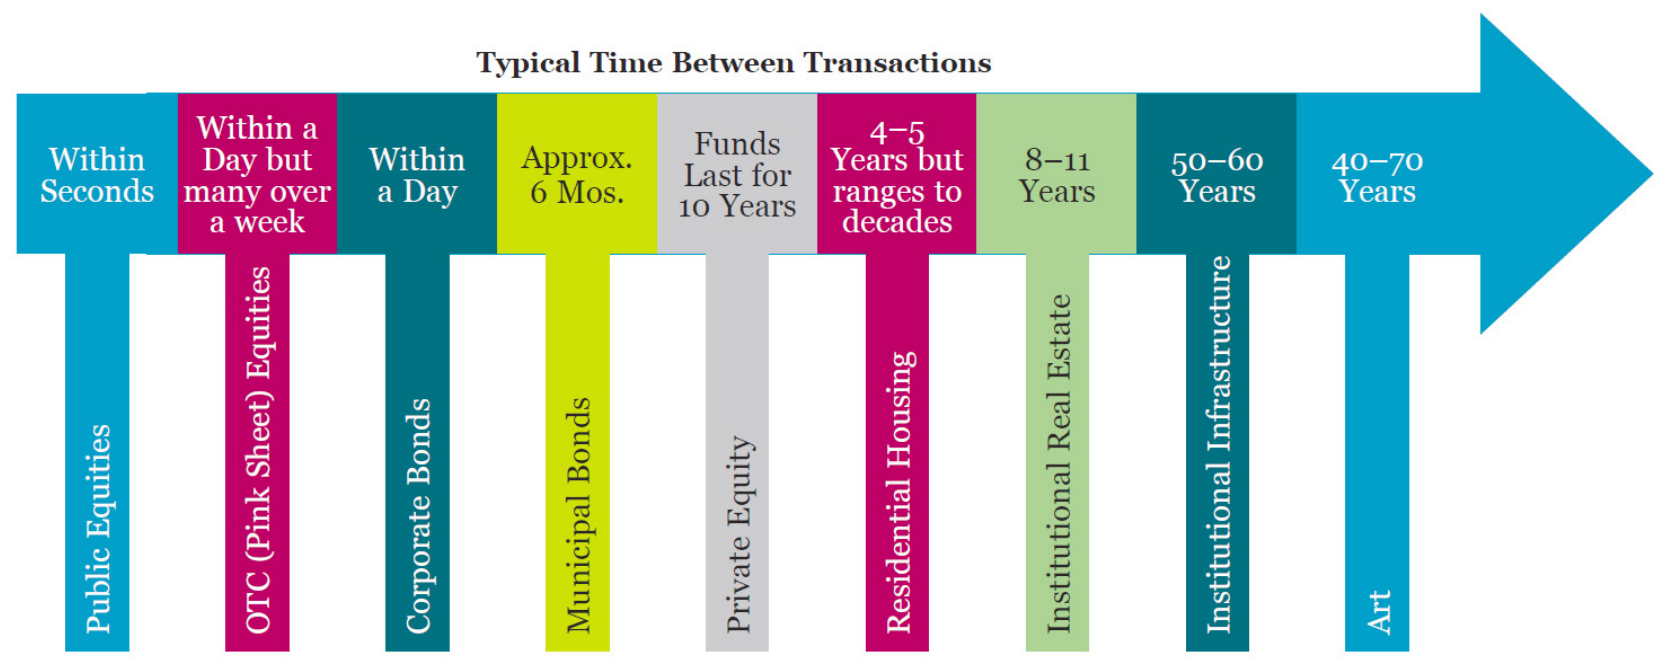
\includegraphics[width=\textwidth]{blackstone.png}
  \caption{Everything Is (Relatively) Liquid\\\textit{Based on \cite{blackstone2015}, source: \cite{ilmanen2011expected}. For illustrative purposes only}}
  \label{fig:blackstone}
\end{figure*}

We see that selling public equities takes several seconds, bonds can be sold within a day, municipal bonds would take weeks or months. Private equities~--- 10 years, real estate~--- 5--10 years, objects of infrastructure such as bridges, roads or factories – tens of years. Works of art may wait for their buyer more than 50 years. 

In this situation, blockchain tokens which can be bought and sold on a decentralized blockchain in less than 10--30 minutes, are an opportunity to tokenize everything that currently takes longer than that to sell. 

The potential tokenization market includes everything that sells over days, weeks or years. Meaning potential for the tokenization market is enormous. The issue currently being addressed by the best blockchains in the world~--- Ethereum and Bitcoin, the issue of having to wait several minutes to receive several transaction confirmations, is no issue to us. 

Asset Tokenization does not work on the market of assets liquid enough to be sold in seconds. The Market Opportunity of BANKEX Asset Tokenization stands to the right of Tokens on Figure~\ref{fig:liquidity-over-time}.

\begin{figure*}
  \centering
  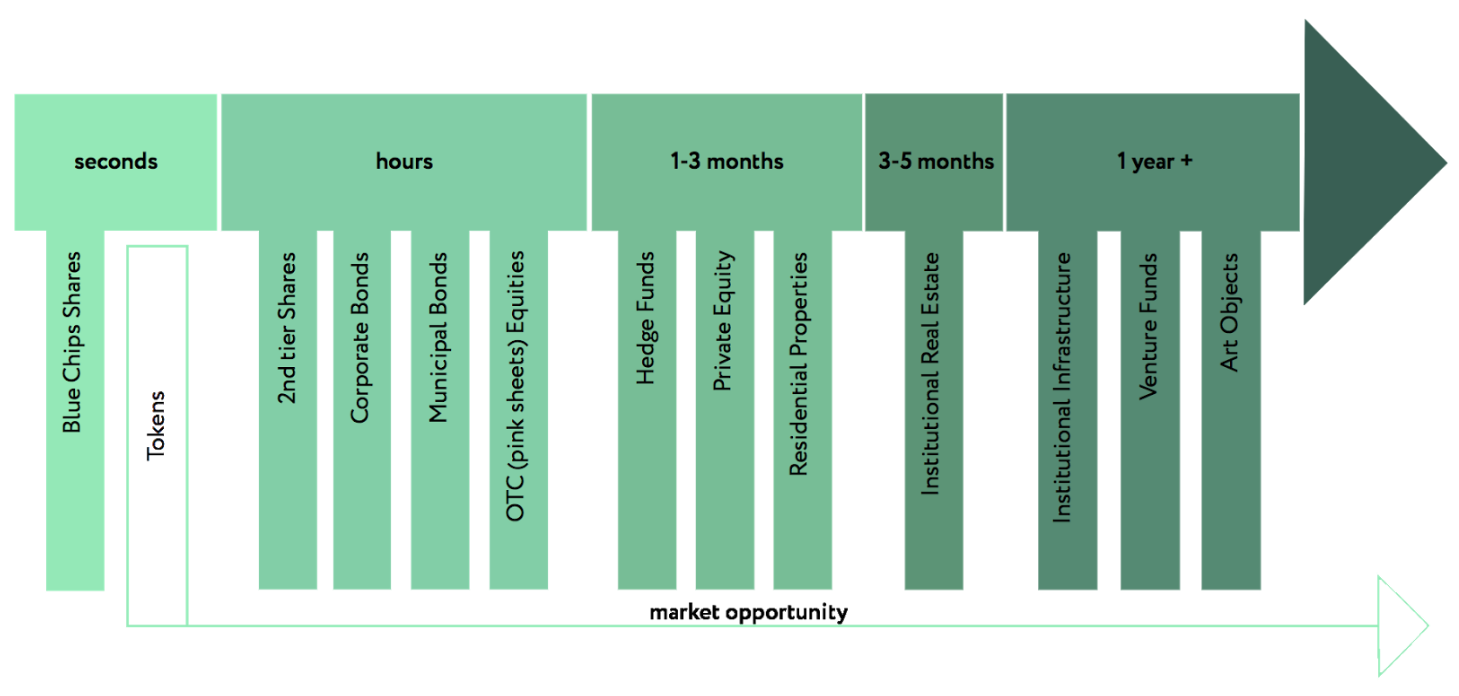
\includegraphics[width=\textwidth]{liquidity-over-time.png}
  \caption{Realizing the Value of Liquid Assets Takes Time}
  \label{fig:liquidity-over-time}
\end{figure*}

We therefore do not compete or fight for the assets that take seconds to sell. This is the market of Ripple\footnote{Ripple provides global financial settlement solutions to enable the world to exchange value like it already exchanges information~--- giving rise to an Internet of Value (IoV). Ripple solutions lower the total cost of settlement by enabling banks to transact directly, instantly and with certainty of settlement. Banks around the world are partnering with Ripple to improve their cross-border payment offerings, and to join the growing, global network of financial institutions and market makers laying the foundation for the Internet of Value. \url{https://ripple.com/xrp/}}~--- the world’s only enterprise blockchain solution for global payments. To them, instantaneous transactions are key, unlike liquidity of Smart Assets during tokenization, where a few seconds don't matter.

In our opinion, target assets for tokenization can include classes of assets with summary capitalization exceeding 100 million USD. 

\subsection{Choosing a Role in New Economy: Coin or Smart Asset}

We receive hundreds of requests: can our business in the real sector be tokenized and how? Many business owners see an opportunity to fund their business using crypto economics via ICO or ITO. Experienced businessmen understand this capital to them is significantly less costly compared to classical sources of capital and is also associated with less administrative risk, as the business decision making center stays in the hands of the owner. In crypto economics there can be no board of directors with members who are non-amicable to you.  

In terms of forming a new economy, BANKEX sees a solution to real business funding in separating technological and infrastructure projects from projects in the field of business operating industrial and manufacturing assets. Technological and infrastructure projects that can help decentralized economy develop and become bigger, more convenient, as well as expand usage of technology over the globe can definitely receive funding via ICO. But what about projects in the real economy segment that require tokenization, but lack strong technological teams, experienced IT founders, financial evangelists?

We all know the crowdsale mechanism will only work with influential founders, powerful ideas and a fully transparent vision of the project’s technological realization.  

The answer is obvious: use the technology and infrastructure of core projects in decentralized economy, including ones utilizing an open source protocol. The BANKEX Proof-of-Asset Protocol is precisely this kind of solution. 

We present to you the procedure of creating a Smart Asset~--- \textit{ISAO} (\textit{Initial Smart Asset Offering}) based on decentralization protocols, such as the BANKEX Proof-of-Asset Protocol. Your asset, even if it’s an offline business, will be able to attract resources by tokenizing its assets using already made powerful technological protocols. You don’t need an ICO procedure, instead you can perform Asset Tokenization of your business using ISAO. 

It’s simple. Use Smart Asset.  

Businesses (farms, stores, manufacturing enterprises) referred to as Smart Assets in our White Paper can be tokenized as part of the ISAO procedure, subsequently forming an \textbf{Asset Community} and receiving returns via Smart Deal.

\subsection{Requirements and Options for Asset Tokenization}

Over the years, working in classic fintech, we have become accustomed to always seek situations that have some sort of problem. Today, we realize that in each of these searches, we would also effectively seek out a problem that prevented an asset from being truly liquid. 

Below are several problems, causing a decrease of an asset’s liquidity, and the more of the below qualities your asset has – the more attractive tokenization of such an asset would be. 

Tokenization of assets gains the greatest value under the following conditions:

\begin{enumerate}[label=(\alph*)]
\item Presence of a large number of asset owners. This means the asset has multiple owners who can have difficulty reaching a consensus. 
\item Distributed asset. You own several office buildings that are rented out several rooms at a time. You can easily see the authenticity of cash flow from the entire asset, but you may find it very difficult, even downright impossible, to figure out the authenticity of cash flow from a single office room. 
\item Standardized end product. This would allow us to identify meta-information when creating a Smart Asset. It’s important for us to be able to bring it to a single basis. 
\item Fungibility (tradability). The possibility of trading one for another. One asset for another asset,  since you as an owner are not concerned with what the asset is. What matters is the cash flow provided by this asset.
\item Use of token as a mean of payment for end-product. An option that would allow the ISAO token released not to be too similar to a payment obligation. A Smart Asset token insures receiving payment, but it can also be used as a means of payment. For example, it can be bought to finance construction of a building, but then this same token can be used to rent a room in this building. As a result, it becomes a utility token, which is important. 
\item Use of the token to own a large asset by a high number of investors and easy means for a buyer to exit co-ownership of a large asset. If an asset can simultaneously be owned by a large number of owners, then it’s makes entry into asset ownership easier. A classical example is shared ownership of large real estate or non-public company shares. Entering such assets with a small share is very complicated at the time.
\item Ability to automatically and unambiguously measure characteristics that directly or indirectly 
indicate a potential quantity and quality of end-products. The ability to integrate regular IoT audit of an asset significantly increases the quality of Smart Asset monitoring. It’s a significant competitive advantage over auditing or rating agencies, whose annual surveys become inferior to real-time IoT audit. 
\item Possibility to withdraw an asset from the owner if the terms of the contract are not fulfilled. This means that, aside from auditing a contract and tokenizing with an escrow module, there is the option of trading the asset, receiving collateral or different contract conditions in the event of a breach of terms. 
\item Control of end-product sales and minimization of the possibility of sales that are not accounted for. This feature does not suit all cases. What this means is that the end product that is tokenized and funded is traced. In the event of tokenizing an agricultural asset such as strawberry, IoT sensors need to be installed that would calculate the number of grown berries to determine whether all of the manufactured berries have brought the appropriate cash flow. These IoT sensors must detect the entire lifetime of an asset up to the generation of cash flow.
\item Assets the transfer of which require high legal and accounting expenditures. Early investors frequently want to sell their assets at the peak of profitability, while other investors are similarly interested in entering ownership of said assets. Tokenization will make such deals significantly simpler and cheaper.
\end{enumerate}

\subsection{Example: Tokenizing Shares in Non-Public Companies}

To give an example of high suitability for tokenization, let us examine late stage private shares that have yet to go public.
These are assets that require very high legal, accounting and administration costs. 

There are many investors in non-public companies who, early ones in particular, are ready to sell their shares, while other investors are interested in entering. But such companies are not public and their shares cannot be traded on the public stock market. Furthermore, they frequently can’t be resold without the approval of company board, since company management must control who their private shareholders are, and prevent their number from exceeding a certain quantity, because otherwise they would breach the limit of investors and become a public company.

These limitations, born from the inefficiency of a historically established system, are an inconvenience to everyone involved~--- both the investors and the company board. In particular, this inefficiency may often lead to disagreements among shareholders and the stalling of company development.

Blockchain technologies allow the necessary details on shares to be recorded in a Smart Contract. Part of the company share, intended for early investors or investors with a miniscule share, is tokenized as an asset in a Smart Asset. Its nominal holder can be any entity permitted by the legislation of the company’s location, such as an SPV. 

After that, from the nominal token-holder’s perspective, they can easily change upon reaching consensus among themselves, as buyers or sellers of tokens of this Smart Asset. At the same time, shareholders are essentially not changing. All presence rights of token holders are passed to the SPV. For non-public companies that don’t want changes in their board of governing shareholders, obtaining liquidity of their capital via tokenization of part of their equity into a Smart Asset is essentially the only mutually acceptable option for all sides involved. 
For early investors this method of investment becomes a new step to decreasing investment risks, and as a result increases the possibility of investment into formerly unavailable assets.

\subsection{Fundamental Advantage of Tokenization for an Asset}

The analytical block of BANKEX, gathering and analyzing financial technologies from all over the world for several years, is seeing an interesting trend that has been forming around financial tools during the last few years. 

If we take apart the basic needs of a person or a company in terms of movement of funds, it would be easy to discover that every person or company does not have that many basic financial needs, namely:
    
\begin{itemize}
\item spending money;
\item moving money;
\item storing money;
\item earning money.
\end{itemize}

By correlating these basic financial needs with the current range of financial technologies it turns out that today there is a strong leaning towards saturation of certain needs with financial technologies:

\begin{itemize}
\item \textbf{spending money}~--- the need that is most saturated and easiest to digitize. There are currently thousands of companies that help a person or a company to easily and quickly spend their money;
\item \textbf{moving money}~--- similar in terms of saturation, but this basic need has several unresolved issues, including ones currently being addressed by our colleagues at Ripple;
\item \textbf{storing money}~--- the need for people and companies to keep their money in their pockets is virtually non-existent today, having fully been digitized and moved to plastic cards and a whole range of innovative solutions. 
\end{itemize}

The BANKEX Proof-of-Asset Protocol allows people and organizations to fulfill an important, vital need~--- the need to earn money. By becoming part of the Asset Community you will have the option of earning, and thus realizing yourself in fields of your choosing. 

Cryptocurrencies solve the global issue of digitization of the human need to earn money, and altogether the emergence of cryptocurrencies is a technological response, solving this fundamental issue. 

SmartDeal based on open source Smart Asset by the Proof-of-Asset Protocol is the next step. You will be able to build your future with your own hands.

\section{Originator, Product Owner and Supplier}

\subsection{Schematic of the Proof-of-Asset Protocol} \label{sec:proof-of-asset-schematic}

In previous sections we have examined the Bank-as-a-Service product model and the concept of Smart Asset Tokenization. These are two big entities, so you may want to know just how BANKEX combines them in its protocol.

The Proof-of-Asset Protocol is the technology for interaction of multiple sides that normally take part in financial deals, but the most important, system-forming sides of the protocol are these three:
	
\begin{itemize}
\item originator;
\item supplier;
\item product owner.
\end{itemize}

Let us examine them using the schematic depicted on the Figure~\ref{fig:asset-bankex-exchange-capital}.

\begin{figure*}
  \centering
  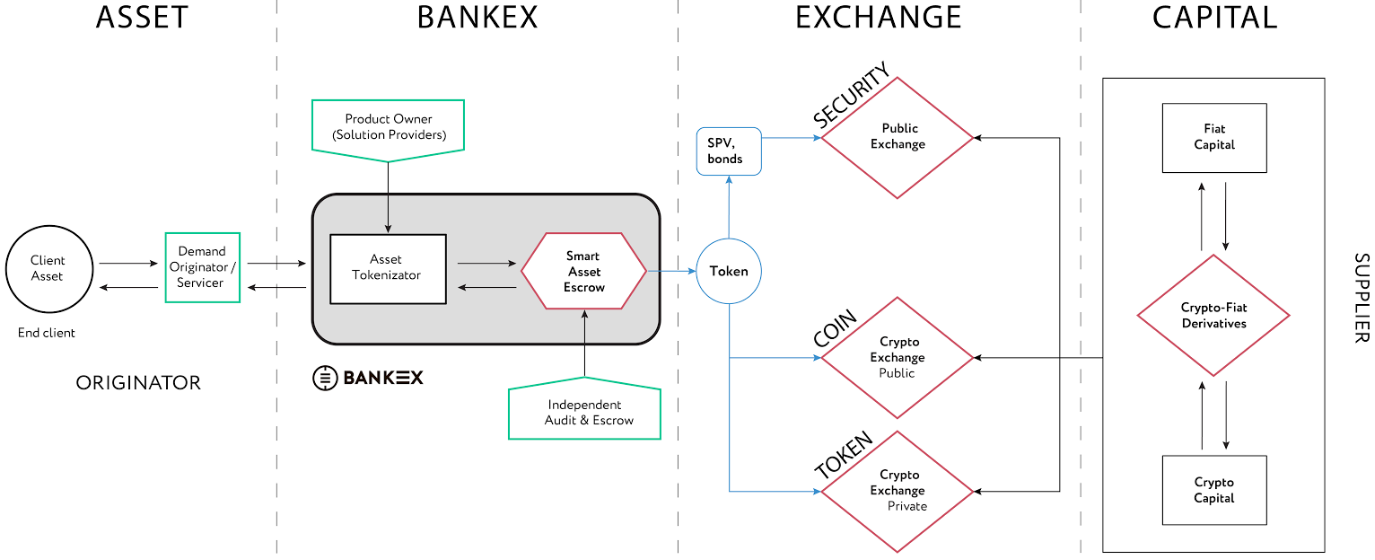
\includegraphics[width=\textwidth]{asset-bankex-exchange-capital.png}
  \caption{Asset~--- BANKEX~--- Exchange~--- Capital}
  \label{fig:asset-bankex-exchange-capital}
\end{figure*}

\subsection{Originator}

On the left side of the schematic is the asset. The originator is the owner of the asset that is being tokenized. The BANKEX protocol allows for the originator to have different roles. On the schematic, for example, the Originator is marked as an end client.

As we've already said, the originator is the owner of the asset tokenized. But despite the originator being the owner of the asset being tokenized, he can also serve as the storefront for products of other originators (types of tokenization - types of Smart Assets). This is something we’ve discussed while examining the BaaS model.

Normally the originator for financial assets is a Bank, but even today it can be an internet-platform (ecosystem), ecommerce, a fintech platform, a stock exchange, a broker, an insurance company. Meaning this is the company the end client goes to, the owner of a client. Anyone can see this almost daily, the simplest example being an IT-company or ecommerce offering their clients more and more new services, including financial ones. They are originators.

It is also fair to assume that there is the option of tokenizing an end client’s assets without the participation of a product storefront. That's why, based on the methodology of processing data in blockchain systems, we define two different types of originators (Figure~\ref{fig:originator}).

\begin{figure*}
  \centering
  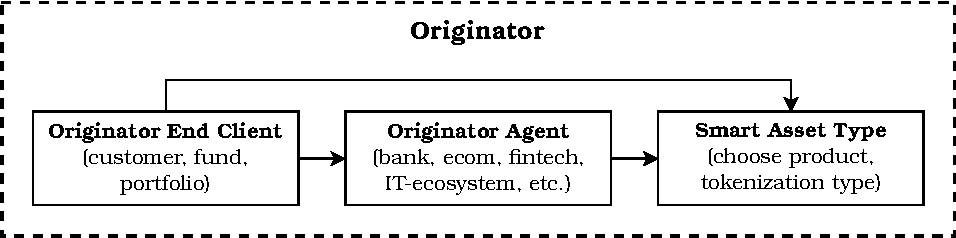
\includegraphics[width=0.6\textwidth]{originator.pdf}
  \caption{Asset Originator}
  \label{fig:originator}
\end{figure*}

\textbf{Originator Agent}~--- an organization (such as a bank), which serves as a storefront for an end client, is the owner of client data or searches for clients wishing to conduct tokenization.

\textbf{Originator End client}~--- an end client wishing to create a Smart Asset in the BANKEX ecosystem, which will be backed by an provided asset.

\subsubsection*{Several important notes}

Both roles can be filled by one and the same organization simultaneously. For instance, a bank tokenizing assets that the bank itself owns. 

From a technological standpoint it is also possible to omit the Originator Agent role in the event of, for example, an end client owning a large asset that they can tokenize themselves. To that end an Originator End client asset needs to have sufficient capitalization. 

For small end clients, work through an Originator Agent is the only possible method to create a liquid Smart Asset. This will be discussed further, as we will examine this very situation in the form of merging requests into portfolios and, possibly, securitization. 

It is also easy to see that tokenization is no threat to Originator Agents, such as banks that are owners of storefronts or end clients, but rather an opportunity for them to provide their end clients with new services and benefits in merging client requests (also similar to securitization).

Thus the Originator in the protocol has the following characteristics:

\begin{itemize}
\item role: creator of the Smart Asset;
\item function: providing asset for tokenization, initiating Smart Asset creation.
\end{itemize}

Here’s a simple example: a small business enterprise (\textit{SME}) \textit{Originator End client} comes to a bank \textit{Originator Agent} wishing to receive a small business enterprise loan \textit{Product (Smart Asset Type)}. The bank has a product: small business enterprise loan \textit{Product Instance 1}, and receives the enterprise’s request. Next the bank has its scoring procedure for this enterprise in order to make a decision on the loan, but the results of scoring mean that the loan cannot be given according to the bank’s rules \textit{Product Instance 1}. The bank automatically checks other available product instances fitting the request and finds an alternative, such as small business crowdfunding \textit{Product Instance 2}, the requirements of which are well suited for \textit{Originator End client}. Then the deal can be made.

As a result, the bank gives the client the product they require, while also keeping their client and satisfying them, instead of turning them down and forcing them to look for a different bank, which may lead to irreversible loss of a client for the bank.

\subsection{Product Owner: Vision}

\textit{Product Owner}~--- a company that creates various fintech products. In the future it will become something more - both the company and the community that create product technologies together.

It's a Solution provider, Product provider and finally Technology Provider. 
Mainly it is a company that owns the technology of Smart Asset creation based on the Blockchain Service Architecture and it creates new types of Smart Assets for the Originator.

At the time of Summer 2017 the BANKEX Proof-of-Asset Protocol ecosystem has two functioning Product Owners~--- daughter company Findelivery\footnote{Findelivery (for Google: Findostavka)~--- fintech company on russian market. The company provides services: delivery of bank cards, remote conclusion of contracts, remote offline KYC clients of the bank. The company has an operating profit. \url{https://findostavka.online/en}} (founded in 2015) and BANKEX~Lab (founded in 2016). It was BANKEX Lab that created the Smart Asset Types that you can try out today by using the tokenization demo \url{https://dev-web-prototype-bankex.azurewebsites.net/}

Obviously the mission of developing and creating all types of SmartAsset the world needs neither can nor should be undertaken by the fintech team of BANKEX Lab alone. That’s why it’s important to us that more and more smart contract developers from banks and fintech companies, as well as blockchain community specialists join the Proof-of-Asset Protocol ecosystem.

BANKEX is creating the protocol architecture with the goal of creating various types of Smart Assets and in our ideal vision of the future, every type of asset will come to have an Asset Community formed for its development, support and audit.

We must note that, for differing locations and jurisdictions the same Smart Asset (Product) would have a differing Product Instance, because for the moment different countries have different laws and legal conditions for transaction processing. This means an enormous number of tasks for developers, for programmers who will be working on the Smart Asset code that will change the way deals are made in the whole world.

Realization of this task is upon the BANKEX Foundation. Every Product Owner can become part of the BANKEX Foundation and make his own contribution to the tokenization of deals worldwide. An important function of the Asset Community in the BANKEX Foundation is support of Product Owners by providing access to product expertise and security audit of the written smart contract code.
CEO of the BANKEX Foundation Petr Korolev\footnote{GitHub of Petr Korolev: \url{https://github.com/skywinder}}, successfully worked with the BANKEX Lab team to develop one of the Product Instances of the protocol in August 2017 at a hackathon. BANKEX’s Ethereum storage of mortgage securities earned BANKEX first prize\footnote{GitHub of the winning solution: \url{https://github.com/BankEx/Blockchain-Hackathon-Kazan}} of the blockchain hackathon from the hands of Ethereum Foundation Council’s Vitalik Buterin. During development the Blockchain Service Architecture methodology was used, which allowed the creation of a superior quality Product Instance from scratch both significantly quicker and more efficiently than other competitors.

It's important to remember that Product Owner, just like separate Product Instances, is a business. A Product Owner can issue Smart Asset tokens, and subsequently provide product expertise, offer audit services or technical support for his Smart Asset Type together with the BANKEX Foundation.

\subsection{Product Owner: Certification}

Obviously, both Product and Product Instances created by the Product Owner based on the Proof-of-Asset Protocol must be certified. This is particularly important for financial Smart Assets. That’s why the ecosystem includes the \textbf{Smart Asset Certification Center} (\textit{SACC}).

The mission of the certification center is to ensure the security of Smart Assets created. Today we can see an industry paradox, which is that the blockchain, created as a technological solution to ensure, first and foremost, the security of transactions, is frequently attacked, and such attacks are occasionally successful. We understand that this is the issue of blockchain technology's rapid development and new solutions must stand the test of time.

To solve this issue BANKEX utilizes the concept of the Smart Asset Certification Center. Its key mission is a synergy of interaction between classical financial institutions and the newest decentralized communities.

This concept is already functioning today. Despite being an innovative approach, we have already turned to it in reality several times. Here's how it works. On the one hand, BANKEX is a classical fintech company, known and valued in many classical banks and financial institutes.On the other hand, founders of BANKEX are all fairly experienced members of the blockchain community. 

This allows synergy when evaluating the Solidity of open source code of new Smart Assets. Here's how it is done currently:

\begin{itemize}
\item first, the Product Owner creates the Smart Asset code and the code goes to BANKEX Lab;
\item next, BANKEX Lab conducts code analysis using in-house programmers;
\item next, even after the brilliant technical expertise of BANKEX Lab's inhouse team, the program code is sent for audit to our partners with old school global technology consultancy, receiving feedback on code quality from top level IT specialists working with leading technological brands in the world; 
\item next step, the updated code is sent to be checked by programmers from several blockchain communities. Their experience is priceless. Almost all of them have had a chance to learn the price of Smart Contract bugs on their own wallets;
\item as the final step of the code audit, the code is validated together with all suggested fixes from all sources by members of the BANKEX Foundation together with the Asset Community and other friendly blockchain foundations.
\end{itemize}

This process may at first glance seem to take more time to validate the Smart Asset code's quality, but when you are steeped in the atmosphere of blockchain research and development, you come to realize that in greenfield smart product development experience of programmers with various training backgrounds allows to achieve impressive results and optimal code quality as quickly as possible.
	
Resulting from the work of the Smart Asset Certification Center, you receive a guarantee of the Smart Asset code's safety from Bankex, a company well known and recognized by the global financial community and listed among the top 50 fintech companies worldwide\footnote{According to \enquote{Top 50 Financial IT Pathfinder Ranking} \cite{top2017}}.

It can be added that the BANKEX team, being a pioneer on the market of legally valid audit of Smart Assets, understands that audit of blockchain-based smart contracts is a new and enormous industry that will augment and possibly replace the existing order of business consulting. We are ready to work in this direction with all players interested in smart contract security, from community teams to consulting leaders.We have no agreements with consulting on paper, but we are negotiating these matters with virtually all the world leaders of consulting and audit, such as Microsoft, E\&Y, PWC, Deloitte and others. Their interest in this topic over the last year has greatly increased and that is the correct approach for everyone.

\subsection{Product Owner: Basic Information}

In the last few segments we have determined the mission of the Product Owner~--- it’s a company that creates various products, meaning types of Smart Assets based on the Proof-of-Asset Protocol.

The Product Owner has the following characteristics in the protocol:

\begin{itemize}
\item role: technology owner;
\item function: to provide technology to Originators in order to tokenize assets. To create various Products and Product Instances on the BANKEX for members of the BANKEX ecosystem. Every Product Owner is a member of the BANKEX Foundation. Products and Product Instances that come from Product Owners must be  certified using the Smart Asset Certification Center.
\end{itemize}

Let us examine the Product Owner from an initial data standpoint using the schematic on Figure~\ref{fig:product-owner}.

\begin{figure*}
  \centering
  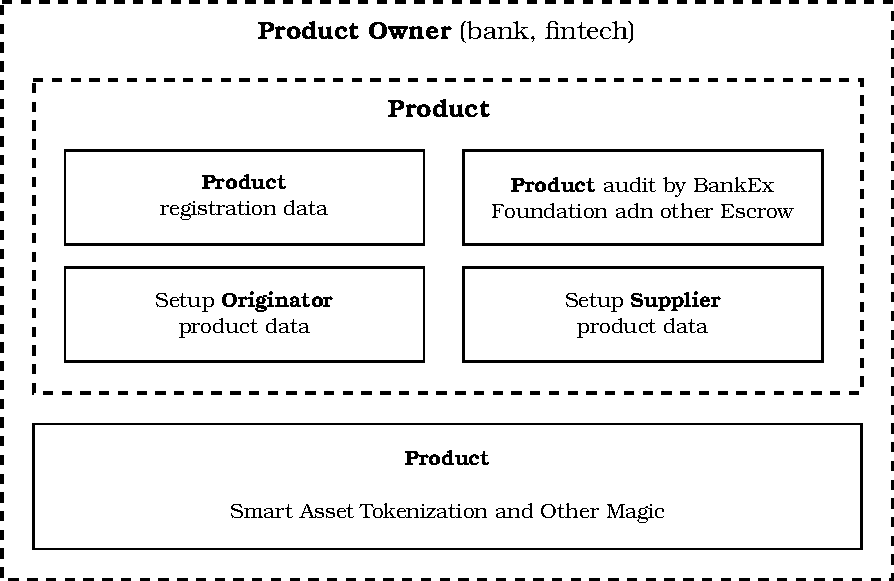
\includegraphics[width=0.6\textwidth]{product-owner.pdf}
  \caption{Product Owner}
  \label{fig:product-owner}
\end{figure*}

A new Product Owner joining the Smart Asset ecosystem must provide basic registration info. To become a member of the BANKEX Foundation this needs to be a company with a registered legal entity and a bank account.

Code of products created by the Product Owner can go not only through a BANKEX audit, but also audit of other organizations and community teams via the Smart Asset Certification Center.

Product~--- a Smart Asset Token, consisting of a chain of smart contracts, based on the Blockchain Service Architecture methodology and the rules of the BANKEX Proof-of-Asset Protocol. The methodology gives the option of creating a Smart Asset on any blockchain, but currently all Smart Assets are being created by the BANKEX team on the Ethereum blockchain. 

Formulas written into the product set the rules for product info that has to be digitized by the Originator and Supplier during tokenization, determining the interconnection between three of the main entities of the protocol.

We call this \enquote{Smart Asset initialization data}.

\subsection{Product Owner: Smart Asset Catalog}

After examining the entity of the Product Owner, we now understand that the Proof-of-Asset Protocol is able to realize a multitude of product solutions and Product Instances depending on application, location and legal conditions. The number of Product Instances is not limited, so to introduce the Product in a new country or account for a change in current legal conditions, the Product Owner needs only update the Smart Asset formulas and releases a new Product Instance. 

With time a large number of Product Instances is going to form for every Smart Asset Type and this number will form a product catalogue that the protocol’s ecosystem will interact with. The BANKEX team calls this the \enquote{\textit{Smart Asset Catalog}}.

Let’s examine how members of the BANKEX ecosystem interact with the Smart Asset Catalog using a schematic. 

As you can see, we have the BANKEX Lab \textit{Product Owner 1}, which, for instance, has created a Smart Asset~--- Blockchain KYC \textit{Product}. This technology is going to be listed in the Smart Asset Catalog \textit{Product Catalog} of the Proof-of-Asset Protocol catalogue. This is very similar to Product Containers utilized in classical banking development.

Let’s say that next two companies came to the ecosystem: Company A from Japan and Company B from USA with the intention to sell the Blockchain KYC technology \textit{Product} in their countries. For these companies and, more importantly, together with them as they have better understanding of the particular traits of business in their country, the BANKEX Lab \textit{Product Owner 1} develops a Blockchain KYC \textit{Product} solution for the Japanese market \textit{Product Instance 1} as well as a solution for the US market \textit{Product Instance 2}.
Next let’s imagine some time after the above a fintech lab called Another Lab \textit{Product Owner 2} develops a Smart Asset for the Blockchain KYC technology \textit{Product}, which gives this technology new consumer features, which could be either superior or inferior to the predecessor. In order to introduce this new technology to the Proof-of-Asset Protocol ecosystem, Another Lab \textit{Product Owner 2} chooses the country and jurisdiction where they wish to apply their solution, and they find an integrator, Company D.

Company D is, for instance, a company on the market of Singapore, where it realizes its solution \textit{Product Instance 3}, which updates the product catalog for the Blockchain KYC technology \textit{Product} with a new instance.

It’s important to note that Smart Asset pioneers who hold the role of Product Owners of their technologies can realize Product Instances for the first solutions on their own, without the need to involve third party integrators. \textbf{Decentralized Product} technology allows to perform integration in the most efficient way possible, skipping steps that would not apply to a particular situation.

Now let's examine the Smart Asset Catalog from a competition standpoint. Obviously instances on markets of different countries will have little to no competition amongst themselves. They are located in different countries the markets of which are, for now, developing independently. But it’s also obvious that Product Owners who harness the technology of building Smart Assets will begin to expand to newer and newer markets, utilizing new integration partners. With the technology developing further there will come a day when several Product Instances form in the same country and the same legal field. This will serve as the push to technological competition between Smart Assets.

There will come a future age of competition between Smart Asset Tokens dedicated to the same Smart Asset Type. In this competition of fully digitized and tokenized assets, the main competitive advantage would be the actual performance of the asset, as well as the outstanding algorithms and value calculation formulas of Smart Assets and subsequent Smart Deals. Competitive advantages of the old world that are achieved through a different kind of benefits will become a thing of the past. This is an enormous quality increase for people in the whole world, as they will have access to assets distinguished by their performance. 

On the side of the BANKEX Proof-of-Asset Protocol ecosystem the Instance Switcher block comes into play, responsible for switching between Product Instances within a single product container. Within the Instance Switcher, Product Instances are processed and arranged, filtered based on various parameters, competing among themselves for buyer requests. Inside the Instance Switcher every product container has its own Instance Trigger that selects optimal Product Instances out of those available for a product based on the criteria set by the client.

Until now we have observed the Smart Asset Catalog top to bottom, from the Product Owner to the Product Catalog, but with the emergence of competing Product Instances the logic of analysis changes instead and we go from bottom to top, seeing the picture of product choice in its entirety. As competition emerges, it's the consumer who determines which Product Instance he will choose, and that is exactly how the process of bidding begins within a single type of Smart Assets. The Instance Switcher can therefore be viewed as an analogue of the classical order book. A buyer's request falls into this order book following the client’s product choice.

This is how a decentralized product exchange begins~--- the Smart Asset Exchange.

\subsection{Supplier}

On the right side of the schematic presented in section \ref{sec:proof-of-asset-schematic} of the Smart White Paper we see the Supplier.
	
The supplier is the owner of the tokenized product.

BANKEX engineers have conducted research of entities and characteristics of resources presently used in various financial and internet ecosystems and have reached amazing results. We have discovered that our typical perception of the resource taking part in deals as financial resource only is too limited.

Perhaps we as a fintech company should be compelled to state here that resource equals money, but our research and development on the matter shows that within the protocol’s ecosystem when creating various types of Smart Assets there will sometimes be Smart Deals with a different resource.

That is why we give the following definition of a \textbf{Supplier End Client}~--- it’s an end client in possession of financial or other resources wishing to use his resource in a chosen Smart Asset to create a Smart Deal with a tokenized cash flow or other goods.

The BANKEX protocol accounts for the possibility that the Supplier may also have various roles, as shown on the schematic on Figure~\ref{fig:supplier}.

\begin{figure*}
  \centering
  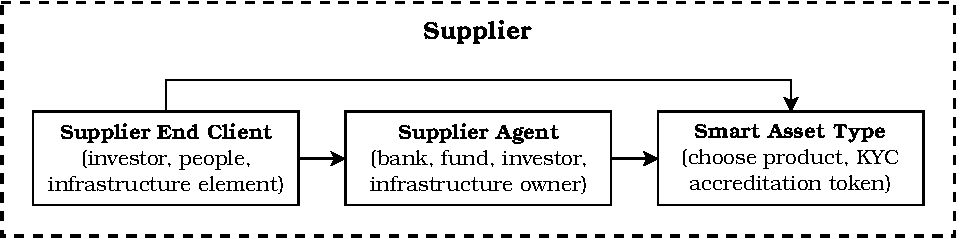
\includegraphics[width=0.6\textwidth]{supplier.pdf}
  \caption{Asset Supplier}
  \label{fig:supplier}
\end{figure*}

\textbf{Supplier Agent}~--- an organization (e.g. bank), representing a portfolio of end clients who wish to take part in a Smart Asset using their resources.

There is a significant difference here from the similar structure of an originator, because in the situation where a Supplier End Client enters the ecosystem without a Supplier Agent, he has no way of accessing a Smart Asset deal directly, instead BANKEX serves the role of a Supplier Agent in this case. Frequently the Supplier will be represented by financial resources, and in order to allow them to enter the Smart Asset Exchange, they will require, at the very least, a KYC procedure of the Supplier End Client based on the requirements of the country where the particular Product Instance functions. That is our current method for our active fintech products. 

For some Smart Assets the BANKEX team develops special procedures of \textbf{Accreditation}. This has to do with the complicated matter of acceptable risk levels for a resource and not all end clients are able to evaluate it accordingly. One of our advisors regarded the development of the Supplier Accreditation procedure as a potential limit to the technology's potential.We are aware that in order to create a global technology, the participants of said technology must not be limited, so the Supplier Accreditation procedure is not a limit. Is it merely one of the smart contracts within the chain of Supplier tokenization and, in the event where a resource is unable to pass Supplier Accreditation, this merely means the Product Owner of this particular Smart Asset needs to determine the ensuing path of the resource tokenized with the new parameters received. This includes determining special legal conditions for it where necessary, if it is required by the country where the Product Instance of the particular Smart Asset functions. This allows to bypass limitations of usage for the Proof-of-Asset Protocol on a low technological level stemming from the particularities of local legislation~--- they are simply included into the tokenization formulas of the corresponding Product Instance.

It is also important to note that, as with the Originator, work through a Supplier Agent is a very simple mean of investing their resource into previously inaccessible types of assets for smaller end clients. End client resources are easily merged into portfolios during tokenization, granting them access to profitable and secure asset types. Never in history have such types of assets been accessible to a simple end client with a moderate amount of resources. Blockchain-based tokenization gives these opportunities to practically any person regardless of accumulated riches or social status. It is a true evolution of liquidity of assets and their accessibility.

So, the characteristics of the Supplier in the protocol are as follows:

\begin{itemize}
\item role: Smart Asset consumer;
\item function: taking part in the Smart Asset and creation of Smart Deal using his resource.
\end{itemize}

\section{Initial Smart Asset Offering (\textit{ISAO})}

\subsection{BANKEX Foundation}

BANKEX Foundation is a non-commercial self-regulated organization with a community the members of which are engaged in work and development of smart contracts for new Smart Assets and Product Instances created with its participation. It includes blockchain technology experts, programmers as well as product providers and product experts.

The BANKEX Foundation as a non-profit organization is an important element of the BANKEX Protocol ecosystem, which allows coordination of the actions of various other elements of the system.

We must note here that while other sections of The Smart White Paper BANKEX describe processes and technologies in various states of readiness but existing in the real world, this section is going to present the model of a concept not yet existing in the world, but aimed at solving issues.

When creating prototypes of various Smart Assets at the BANKEX Lab we have encountered a situation where many business owners from various countries started coming to us, wishing to tokenize their assets via the ICO procedure. Our vision of tokenization, which we have already discussed in this White Paper earlier, concludes that issuing your own coin is a poor solution for assets belonging to the real sector of economy where rocket science technologies don’t exist. Nonetheless, the necessity and even inevitability of the tokenization of their assets in the future are obvious. We suggested the procedure of Smart Asset emission to these clients, some of the resulting Originators were accepted by the BANKEX Lab as pilot designs. These assets will be prepared for the \textit{Initial Smart Asset Offering} (\textit{ISAO}) in the Proof-of-Asset Protocol ecosystem. But we turned down the majority of them.

How do we see the possibility of providing these businesses with the option to tokenize, regardless of the centralized initiator-company of the Smart Asset?

The BANKEX team assumes the Market will form more and more such requests as time passes. These requests will come from owners of businesses or assets, meaning Originators with No token Asset. The BANKEX Lab is receiving such requests now, but subsequently they will be addressed to multiple Product Owners in the ecosystem. Those requests that the Product Owners can tokenize they will process, creating Product Instances. Of course, they will also turn down many incoming requests. The reason is not so important at this point.

Such requests for tokenization of a new type of assets are directed by acting Product Owners to the BANKEX Foundation (Figure~\ref{fig:isao}). 

\begin{figure*}
  \centering
  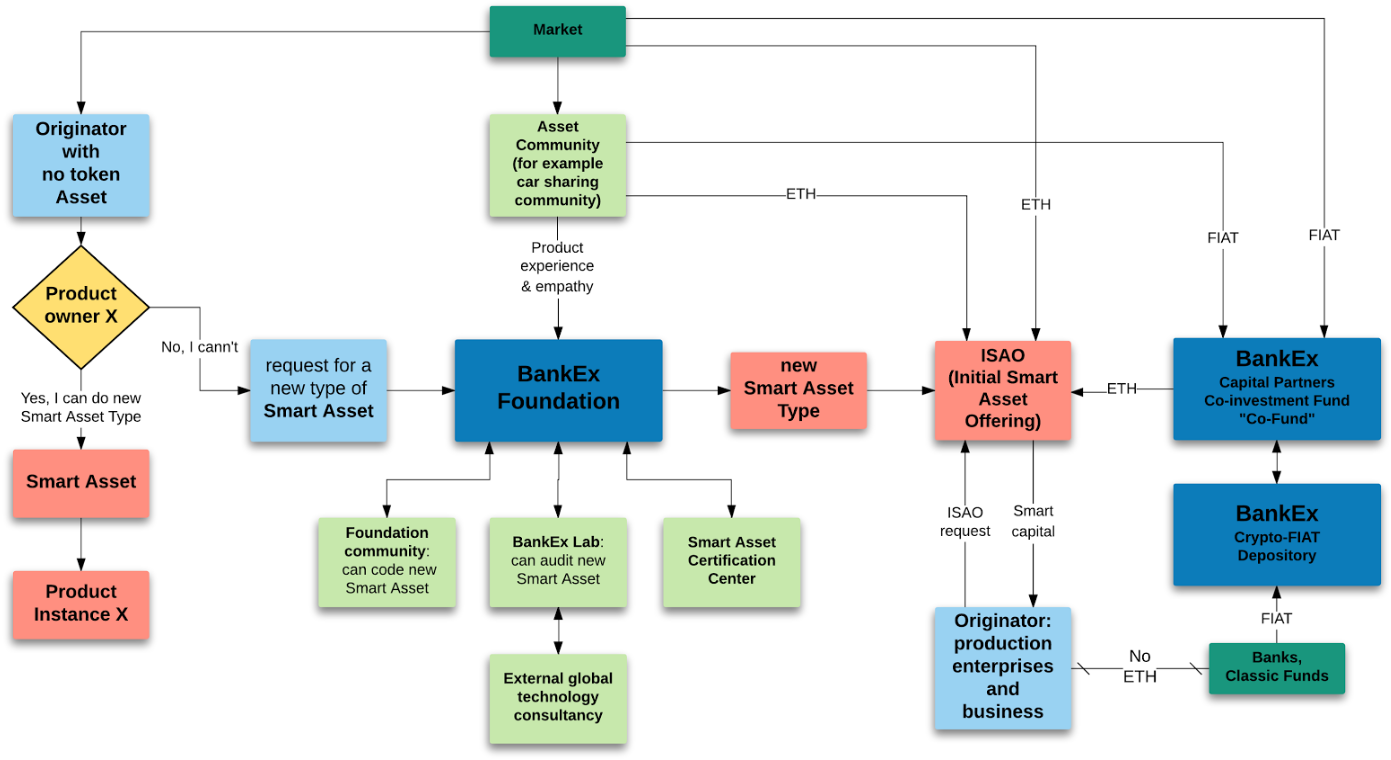
\includegraphics[width=\textwidth]{isao}
  \caption{ISAO Structure}
  \label{fig:isao}
\end{figure*}

Now let’s examine the schematic to see how the BANKEX Foundation coordinates actions:

\begin{description}

\item[Asset Community]--- as the request for creation of a Smart Asset came from the Market, there is clearly an individual or group of individuals who are pioneers and enthusiasts of this product. These are the people the BANKEX Foundation forms a product community from for the creation of a new type of Smart Asset. This product community then takes over the business development of the aforementioned Smart Asset. The initiator of the request for such a Smart Asset Type may become the founder of said Asset Community. Such communities are also needed by the ecosystem for two more important functions - product expertise and providing Proof-of-Asset evidence in the event of Smart Deal disputes. It’s important that in the Asset Community we do not require identification of all the members~--- they take part in the ecosystem only with their knowledge and experience. 
\item[Foundation Community]--- this is a community of programmers and business developers, who are fans of the decentralized Blockchain Service Architecture. They are the people responsible for creating the world-changing chains of Smart Contracts for various No token Assets.
\item[New Smart Asset Type]--- is a program code fully ready for initiation. As we see on the schematic the Asset Community, Foundation Community and the BANKEX Lab with participation from third party experts takes part in the creation of this code. The quality of the code is guaranteed by the BANKEX Smart Asset Certification Center.
\end{description}

So the BANKEX Foundation in the protocol has the following characteristics:

\begin{itemize}
\item role: community built around the protocol;
\item function: creation of new types of Smart Assets and the development of the protocol that will be in-demand by the community, as well as the growth of the community that is going to use the protocol.
\end{itemize}

\subsection{BANKEX Crypto-FIAT Depository}

One of the existing and not yet solved issues in asset tokenization is the impossibility for legally significant organizations to purchase tokens. There is a long series of details relevant for different locations.

Let us pause on the most important and define their common features.

First, banks and organizations are able to invest into companies, using stocks and equities. In banks, classical funds and large financial groups there are special departments that invest into corporate securities and other financial instruments on stock exchanges. These departments are able to invest into securities, but lack the ability to invest into cryptographic coins and tokens, as they have no common tools for that.

Second, banks and organizations must place purchased assets on their balance upon investment, for that they require legally relevant documents that confirm purchase of the asset. Token purchase provides no such documents. 

Third, banks and organizations lack the technology to follow their existing security regulations when storing cryptoassets. As we all know, should the private key be compromised, that would be enough to lose access to the crypto wallet, and it doesn’t matter what amount is stored on the wallet, if a malignant party obtains the private key it can vanish in an instance. Banks are unable, or rather they cannot permit assets to be stored with such security parameters. 

In the BANKEX ecosystem solution of these problems is handled by the \textbf{BANKEX Crypto-FIAT Depository}. This is a legal organization and a technology for cryptoasset storage. The Crypto-FIAT Depository works as any classical depository with the only difference being that it grants its classical clients the ability to store cryptoassets.

We see this as the Depository forming a legal agreement with a bank or organization to give the Depository permission to store clients’ cryptoassets. After that the client registers a wallet in the Depository for the cryptoassets he requires. If it’s an ERC20 token then an Ethereum Wallet is registered. After that the client does not receive the private key to the wallet - instead it’s instantly conserved in the depository’s storage until the client closes the account. The client receives a regular depository receipt in return for his cryptoasset.

The technology to store coins and tokens in the Crypto-FIAT Depository allows a client to conduct operations with cryptoassets on his balance, and what’s more important, it lets him do this in a way that he’s used to. He sees these cryptocurrencies in the same way he would see classical assets. This is the very technology that FIAT and Crypto markets are waiting for.

\subsection{BANKEX Crypto Fund}

\text{}

\subsection{Initial Smart Asset Offering (ISAO)}

Initial Smart Asset Offering (ISAO)~--- is the initial Smart Asset offer with the goal of tokenizing financial assets or real economy sector assets in the form of emission and sale of Smart Asset Tokens to buyers.

An ISAO can only be carried out with an asset present, in other words either a functioning or planned cash flow. A technological startup or RnD cannot be tokenized via the ISAO procedure.

On the schematic (Figure~\ref{fig:isao}) we can see the request for an ISAO comes from an Originator, i.e. owner of a financial or manufacturing asset. This Originator does not need to create the tokenization technology~-- instead the best programmers from various teams coordinated by the BANKEX Foundation compete for its creation.

It would be fair to state that a first-time Originator with the desire to create a new type of Smart Asset and an Originator initiating an Initial Smart Asset Offering can be one and the same person, which is what we are striving for. But at the same time this schematic does not permit centralization of the program solution, as the Originator neither influences the actual writing of the Smart Asset code, nor controls the programmers, the Originator is only able to take part in the development via product expertise using the Asset Community mechanism. 

In the BANKEX Proof-of-Asset Protocol ecosystem the following can take part in the initial purchase of Smart Asset Tokens on a technological level:

\begin{itemize}
\item buyers originating from the market;
\item banks and classical funds via the BANKEX CF Depository and “Co-Fund” systems;
\item members of the product community interested in development of assets of this particular type.
\end{itemize}

If the buyer originates from the market or the Asset Community and he needs to make a purchase using FIAT currencies, he has the ability to do that via the Crypto-FIAT Depository. If the buyer wants to make a purchase using ETH~--- he can do so directly.
	
The buyer of Smart Asset Tokens~--- in terms of entities present in the Proof-of-Asset Protocol, as outlined in the previous chapter~--- takes the role of the Supplier.

\subsection{Open Source: Smart Asset Core}

BANKEX Foundation presents a platform for collaborative work with an open source code, created to promote technologies in the banking and financial sectors.

An Open Source approach to development based on collaborative use of software can ensure transparency, stability and support needed to implement blockchain technologies. The main task of organizations is the development of a global cooperation and support of leaders and entrepreneurs in the field of finances, banking, Internet of Things and decentralized technologies. 

We welcome all who take part in the developer community of the Smart Asset Protocol regardless of membership status. Additional information on the technical details and methods of collaboration can be found on the community page \url{https://github.com/BankEx}.

Open Source Protocol~--- Smart Asset Core (\url{https://github.com/BankEx/smart-asset-core}) is the base structure to tokenize and securitize assets. It contains all the necessary modules for integration of third party information providers and tools for writing specialized smart contracts.
	
\subsubsection*{Open Source Proposal:}

\begin{itemize}
\item development of the blockchain community in order to support the Proof-of-Asset Protocol;
\item establishing partner connections and their subsequent technical support;
\item formulation of the direction of technological development and establishing interaction with Product Providers;
\item creation of the protocol’s core architecture with subsequent increase of functionality by involving specialists from the open source community;
\item ensuring protocol security, including by means of involving third party white hat hackers \& developers;
\item organization of a tight cooperation with solutions of other open source communities, such as the Consensus Foundation, Ethereum Foundation, Symphony Foundation, Hyperledger
\end{itemize}
	
\subsubsection*{Open Source Finance part:}

\begin{itemize}
\item tech support for partners;
\item bounty program for developers (expenses)~--- guarantee of security.
\end{itemize}

\section{BANKEX Proof-of-Asset Protocol}

\subsection{Registration data \& product data}

The our first step in researching the liquidity protocol is data. BANKEX as a classical fintech company is well aware how many different existing banking systems there are, many with an architecture that was established many years ago.

That’s why in order to build the protocol technology we have begun our research from scratch, rather than basing it off of any existing IT infrasctructure of a bank. This may be an unexpected decision to some IT specialists of the banking segment, but we have decided to separate all the information we work with during initialization of Smart Assets into just two parts: registration data and product data. We see no reason to overcomplicate this.

Registration data~--- data that allows the identification of a client. Modern registration data contains an intrinsic fundamental controversy. On the one hand, internet platforms have evolved to the highest level of simplification for this data - most of them request nothing but a client’s e-mail upon initial registration. On the other hand, in order to work with financial information in global economy, it is necessary to receive the most extensive registration data from the client - this is a matter of public security.

In the blockchain network technology there is, in essence, only one vitally important identification, which is the address of one's wallet. As we are building the financial asset tokenization protocol, we find this information insufficient. 
Here is our solution. The registration data that allows client identification is taken beyond the tokenization cycle. When a Smart Asset is created on the Ethereum blockchain, we retain the technological capability to perform tokenization using only the Ethereum Wallet number, but at the same time we also create a connection between the Ethereum Wallet used in tokenization and the other registration data using the BANKEX KYC Adapter. This is imperative as different banks may have completely different assortments of client registration data and, what’s more important, these are personal details that are protected in many countries. It would be unwise to create a Smart Asset reliant on them. 

On a technological level the Proof-of-Asset Protocol allows the BANKEX KYC Adapter to be integrated with any KYC provider functioning in the country. BANKEX has a subsidiary with a working product of this type. This is not rocket science. All we can say is we are followers of the technology of client identification via blockchain-stored hash, received from client data initially verified by a reliable source. 

The most important consequence of the decision to take registration data beyond the tokenization cycle using the BANKEX KYC Adapter, is that various Originators, including banks, can now be integrated more comprehensively and with minimal effort. The Originator defines identification parameters and the Proof-of-Asset Protocol adjusts to suit those parameters, creating a link between client data and the Smart Asset blockchain wallet. 

What about the data that goes into the Smart Asset? That's product data - an arrangement of data necessary to tokenize the client’s asset, with parameters and contents defined exclusively by the Product Owner separately for every Smart Asset Type. 

On the schematic you can see, along with the protocol entities you have already become familiarized with, that the Product segment includes blocks that define product data for both the Originator and the Supplier.

The quantity and types of product data fields are not limited in any way~--- it is decided entirely by the Smart Contract logic necessary for a particular Product Instance. 

As a brief summary, the ecosystem of the protocol generally allows for various other registration data~--- the principle of work with them is always going to remain unchanged, they are technically impossible to store in a Smart Asset. In any event where any entity needs to be identified, the process of identification itself is always going to be beyond the logical cycle of the Smart Contracts included in the Smart Asset. The protocol only interacts with such data on the level of confirmed or unconfirmed registration data hashes that come from external oracles. 

The only possible exception to this rule is when the Smart Asset Proof-of-Asset Protocol is fully realized on the Microsoft Azure Bank API server within the bank’s security network.

\subsection{Creating a Smart Asset}

As we have already discussed the Blockchain Service Architecture allows formation of various chains of smart contracts based on the protocol. Let's examine the order in which a typical Smart Asset is created.

We see five desired logical steps in the Proof-of-Asset Protocol to be able to call a token a Smart Asset (Figure~\ref{fig:poa-protocol}). These steps are:

\begin{itemize}
\item initial contract;
\item validation;
\item audit;
\item legal;
\item proposal.
\end{itemize}

\begin{figure*}
  \centering
  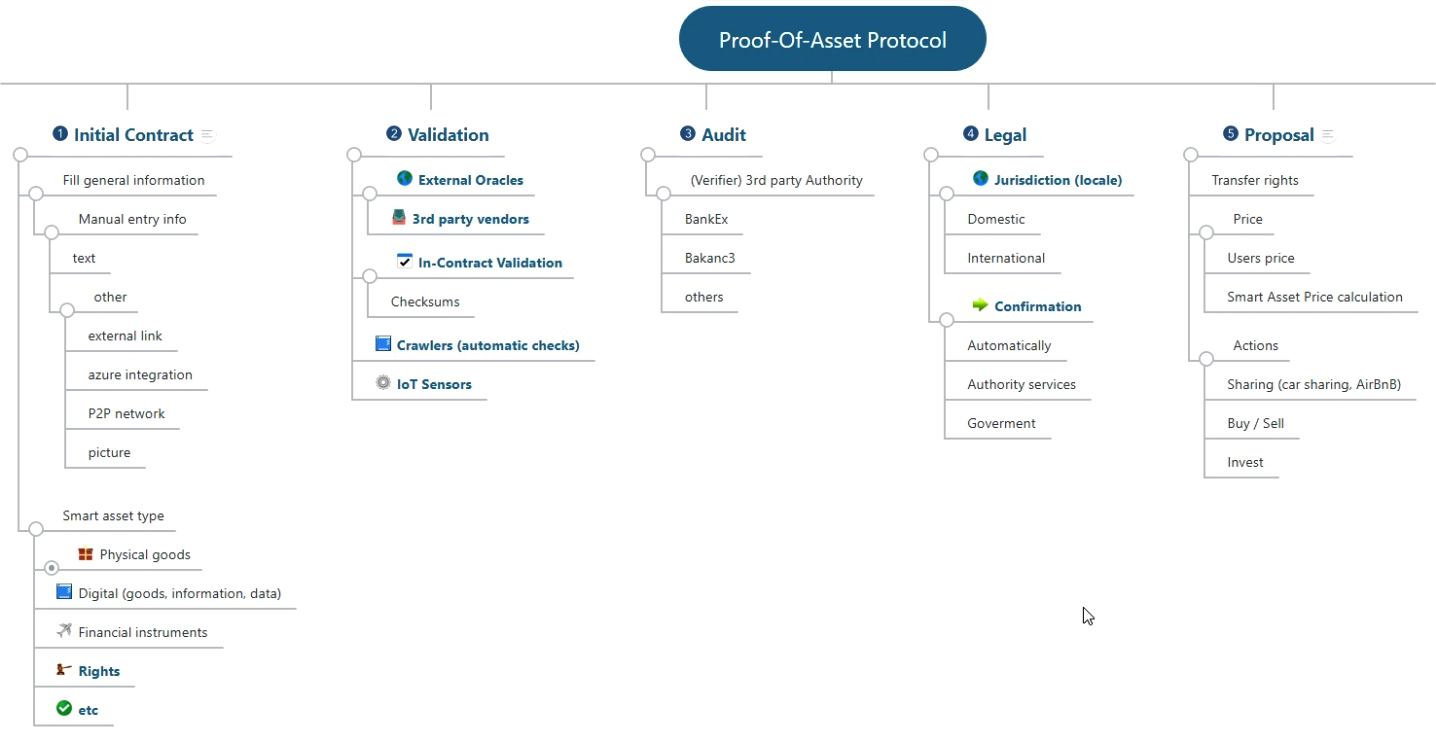
\includegraphics[width=\textwidth]{poa-protocol.png}
  \caption{Proof-of-Asset Protocol}
  \label{fig:poa-protocol}
\end{figure*}

We first initialize the contract, selecting a type of Smart Asset. The Smart Asset’s type determines product data required for the token and the logic by which that data is processed. 
Next the Originator fills in General Information, which can happen both manually and automatically. Data entered by the Originator is what we presently call digitalization. The information is there, but its value is unknown as the filled in forms have no function and, more importantly, have no validity - we have no way of knowing if that information is genuine. 
The next step is Validation. This is where Smart Contracts are executed that validate the information entered by the client using various trusted sources. These can include Internet of Things Sensors, Eternal Oracle, Crawlers and others. It is crucial that the contract is saturated with data from sources independent from the Originator, which allows for an accurate assessment of the authenticity of General Information provided. 

Next the result is audited, always by an outside party. This is the part of tokenization where a 3rd party gets involved. Primarily this is BANKEX, comparing hash totals of the current Smart Asset code with certification data from the BANKEX Foundation. Only a verified SACC code can get the BANKEX Verifed mark. These can also be accounting services or any other services that can check the process of tokenization based on Smart Asset logic.

It is also important that at this point classical offchain organizations can also get involved, if that is supported by the issuing conditions of the Smart Asset. 

Legal is the step where every Product Instance can set up legal conditions specifically required for both it and the country where it's located. This is also where the Smart Assets intended for global liquidity establish the norms of governmental and customs regulations. The Blockchain Service Architecture allows any existing legal regulations to be written into Smart logic. If the government of your country demands that you must receive an official document from the town hall for your asset, then you do just that. You head to the town hall, receive the official document, scan it and add it into the Smart Asset with your signature or that of a certifying officer. After the government implements tokenization to their algorithms you can simply change the one corresponding Smart Contract included in your Smart Asset. 

Proposal~--- Smart Contracts that fix the base price of a Smart Asset and define the type of operation that will be performed with the taken asset on the Smart Asset Exchange. From a stock exchange perspective, the result of this step is the creation of a bid. From a blockchain perspective~--- the issuing of a token.

\subsection{Smart Asset Сaterpillar}

The BANKEX team named this tokenization principle the Smart Asset Caterpillar, although it was not our first choice of name. It was picked up when we realized that in order to achieve true value of a Smart Asset, which means proving that it is ensured by an actual asset, it was imperative that smart contracts in the chain were to flow from one to another in an uninterrupted sequence. If you were to cut an earthworm in half, its parts will survive for a time. But if a caterpillar is cut in half or even if it loses any segment of its body~--- it dies. This principle is true for the Smart Contract chain in a Smart Asset. If you interrupt the chain or either of the links becomes invalid then the Smart Asset formula will result in a value of zero for the asset. Any link of the Smart Asset Сaterpillar being insufficiently validated would have a detrimental effect on the resulting value of the entire Smart Asset. 

A second important consequence of the Smart Asset Caterpillar tokenization principle is that every significant step on the chain that affects the Smart Asset’s value is recorded on the blockchain. You enter your General Information during step one and press next - the Blockchain Service Architecture asks if you wish to record your commitment on the blockchain (Figure~\ref{fig:asset-creation}), after which you will receive details of the transaction on blockchain (Figure~\ref{fig:asset-detail}).

\begin{figure*}
  \centering
  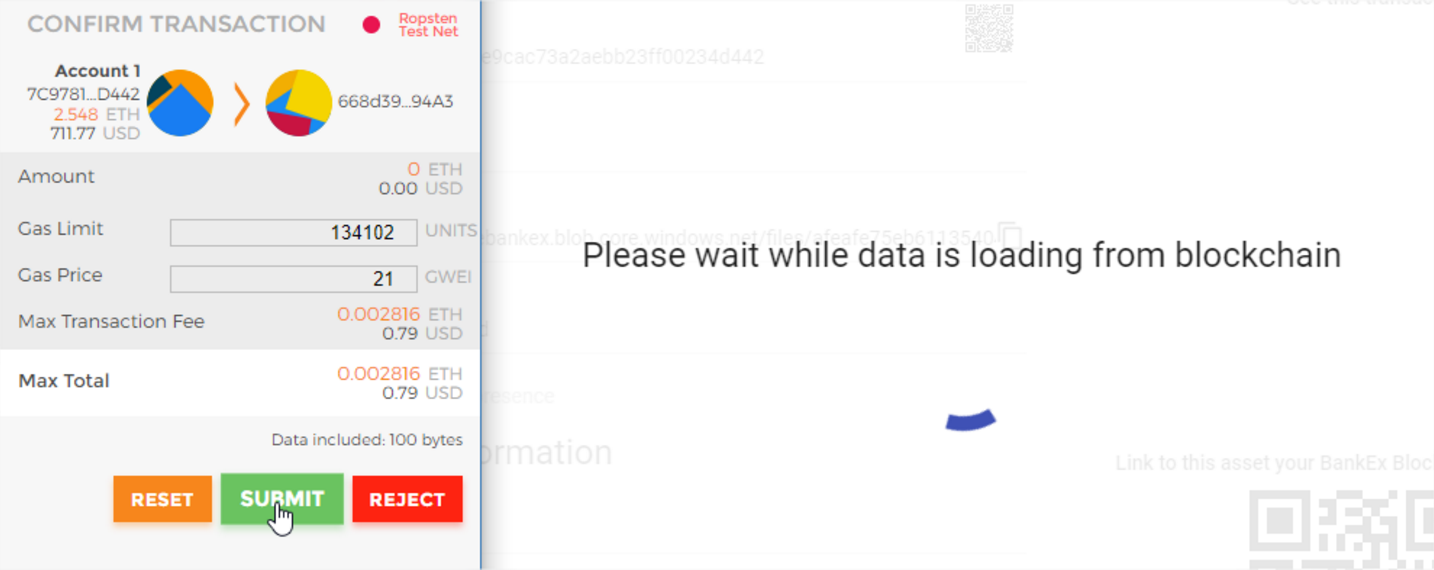
\includegraphics[width=0.7\textwidth]{asset-creation.png}
  \caption{Step~1~--- Asset Initialization}
  \label{fig:asset-creation}
\end{figure*}

\begin{figure*}
  \centering
  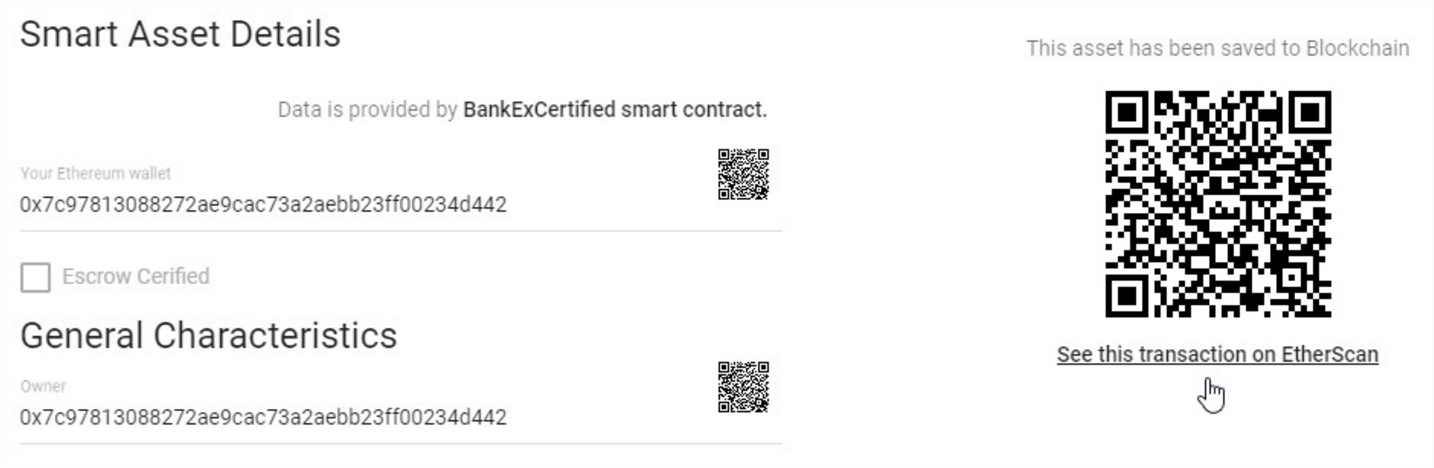
\includegraphics[width=0.7\textwidth]{asset-detail}
  \caption{Step~2~--- Asset Validation}
  \label{fig:asset-detail}
\end{figure*}

This is not just digitization~--- it is tokenization, an imprint of your commitment and, the further along the Smart Asset Caterpillar you are, the more valid your commitment is to other members of the ecosystem.

It's worth noting here that the BANKEX Proof-of-Asset Protocol technology supports several technical solutions for the recording of the aforementioned imprints on the blockchain, including industry-specific know-how. 

\subsection{Initial contract}

The exact way in which every contract is initialized is defined by the Product Owner when calculating the Product Instance (Figure~\ref{fig:initial-contract}). Let us note several significant steps for the majority of Smart Assets.

\begin{figure*}
  \centering
  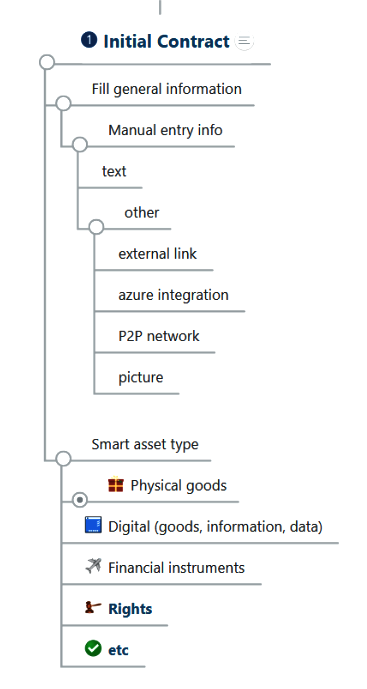
\includegraphics[width=0.4\textwidth]{initial-contract.png}
  \caption{Initial Contract}
  \label{fig:initial-contract}
\end{figure*}

First, initialization will require the registration data of the Originator End Client, and as we operate in the technological stack of the blockchain network, we have agreed not to store registration data~--- we must receive a Wallet address. For the demo version of our product we used a web interface with the Metamask Ethereum Wallet plugin (Figure~\ref{fig:originator-client-kyc}):

\begin{figure*}
  \centering
  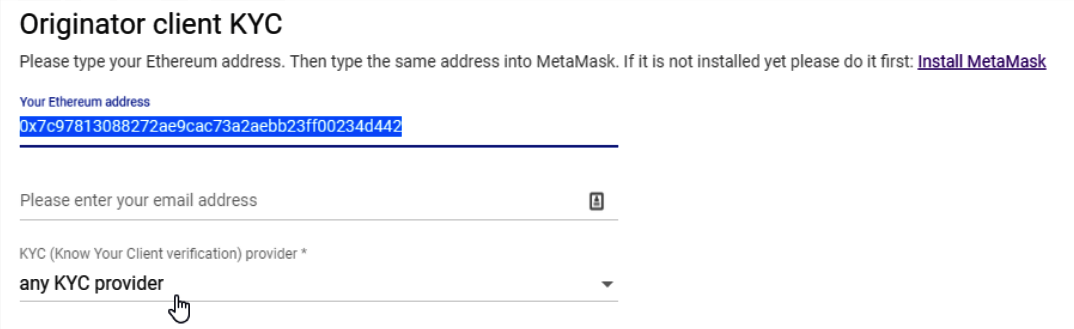
\includegraphics[width=0.7\textwidth]{originator-client-kyc.png}
  \caption{Example of Asset Initialization}
  \label{fig:originator-client-kyc}
\end{figure*}

With this iteration the Ethereum wallet address is automatically taken from the plugin. In other iterations or on other blockchains this may work differently.

Why do we need a wallet address? By using it we receive the ability to perform client identification through the BANKEX KYC Adapter or any other KYC provider. Additionally, the demo shows it's possible to request an optional field as well, such as an e-mail. 

Second, when initializing the contract data is entered into General Information fields. General information is entered either manually by the client or automatically, but its accuracy is decided only by the person inputting it. It would be fair to state that tokenization does not rely on accuracy of the General Information entered. We take it as it is, whereas the authenticity required for the Smart Asset is going to be determined by the logic of subsequent contracts in the chain. It's interesting that not all true information may actually be required by the Smart Asset, and an Originator End client who doesn't know how to determine a code's Solidity may not even know how important the fields he is filling in are. When the BANKEX team hears talk about the need for each and every person in the future to have programming skills, we immediately recall our Smart Asset Caterpillar.

Third, in the General Information block of the demo we show that information fields may be of any type, depending on the habits of a programmer. A type-bar, a file, a catalogue, digits~--- any type of field at all. 

Fourth, part of the General Information block's function may be carried outside the blockchain logic and outside the logic of external oracles, instead being based on the UI alone. Our RnD showed that the simplest but sometimes necessary function of the logic, such as checking hash totals in specific fields can easily be diverted to web-based or any other programming logic used in a particular Product Instance. 

The results of the Initial contract steps are:

\begin{itemize}
\item creation of a Smart Asset entity;
\item assigning the Smart Asset with a unique ID for subsequent connection IoT and Oracle;
\item may involve the creation of a legal Soft Commitment;
\item a data record on the blockchain.
\end{itemize}

\subsection{Validation}

The Validation step (Figure~\ref{fig:validation}) of a Smart Asset is the most fascinating for Research and Development, this is where various means and methods for the validation of the General Information can be built.

\begin{figure*}
  \centering
  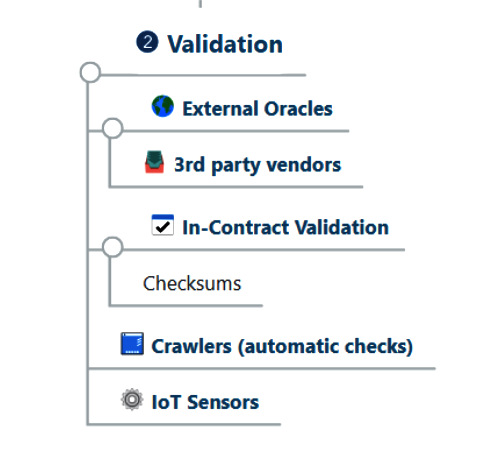
\includegraphics[width=0.4\textwidth]{validation.png}
  \caption{Validation Step}
  \label{fig:validation}
\end{figure*}

Let us define the following terms.

\textbf{Internet of Things} (\textit{IoT}) will be the main condition for the validation of Smart Contracts, and this will come much sooner than we can imagine. Very soon our world will become filled with myriads of various sensors and transmitters for smart contracts, just as it has already become filled with smartphones and surveillance cameras. 

IoT Sensors can come in any number of different combinations. BANKEX is not an IoT company, and yet our lab already has more than 50 different sensors with different purposes. In the demo application we used three of them - an accelerometer, a location pin and a photo camera that any smartphone is equipped with. Let us remind you here that cell phones are already used as tools for payment. 

Many companies today are trying to create Smart sensors, outfitted with an internal logic, but the decisive potential is definitely held in a combination of IoT Sensors and the logic of Smart Assets. 

The second element are \textbf{External Oracles}, which are the obvious choice for data validation today, and which are used by many companies worldwide. You can check a person’s information using his Pass ID or request information on an organization using its Registration Number. You can request information on rates and constants being developed by public organizations or institutes. Or you can simply perform crawling of information from a chosen website. Everything you need for your Product Instance. Using External Oracles it's possible to implement almost any logic you could need on the Ethereum blockchain even today, it's not complicated.

Use of the oracle technology to examine images or videos captured by IoT sensors deserves additional mention. Soon enough you will not have to pay for the recognition of your car license plate. The Smart Contract would be able to send a fine from your bank account on its own. 

Smart Asset creation logic may include any number of External Oracles and each calculation will have its price, but even today there are technical solutions which allow them to be cheapened on the Ethereum blockchain. It would be safe to assume that in the future there will likely be even more such solutions available.

Internal checks are simplest logical flags or hash totals that nonetheless may greatly impact the price of a Smart Asset, for instance a flag showing whether or not there is a supporting document uploaded along with the request to the Microsoft Azure cloud. 

The results of the Validation step are:

\begin{itemize}
\item additional information input into the Smart Asset entity;
\item formula determining the importance of concluded validation;
\item operation saved on blockchain.
\end{itemize}

\subsection{Audit \& Legal}

In terms of technical implementation, interaction with third party audit organizations, jurisprudence or government is also dedicated to an External Oracle.

We initially called this section Global Delivery Conditions because in order to make an asset as liquid as possible, it must achieve global liquidity. It is similar to Amazon.com in the field of digitized goods. Global liquidity of various assets is our future, now the most important task is the embedding of the Smart Asset ecosystem into existing national legislation and state regulations. 

We are often told that the implementation of Smart Assets is extremely complicated due to the impossibility of giving them legal significance. It’s true that it’s a complicated task, but offchain legal conditions are not at all difficult to write into the chain of Smart Asset contracts, even if one of the Smart Contracts requires action to be taken offchain or even offline. Does something need to be done and then marked with a tick? Good - we include this condition into the logic of the Smart Asset’s function and mark it with the tick, then the Smart Asset becomes valid and, consequently, gains value. 

Obviously, the implementation of Smart Contracts is only a matter of time for any efficient nation, since the volume of inefficiencies in any large organization, including nations, is enormous. It is both beneficial and sensible. Once a nation’s work conditions are modernized, you need only update your contract chain to the latest Product Instance. In fact, if you are the Originator, you won’t even have to do that~--- it will be done by the BANKEX Foundation. 

Cost of delivery estimation and automatic customs tax of the exported asset based on data from the location sensor could also occur during this block. Which, we may add, opens the way for export/import of cash flow associated with various types of assets between nations. 

\subsection{Proposal}

Logically and technically this is the most difficult step of the Smart Asset Сaterpillar. 
It’s where the magic happens:

\begin{itemize}
\item trading rules are set for the chosen type of Smart Asset;
\item asset authenticity rate is calculated;
\item the asset's base price is calculated;
\item the asset's intended use is specified;
\item Hard Commitment parameters are set;
\item cash flow distribution is defined according to Smart Deal.
\end{itemize}

Actually everything is much simpler, with complicated deals that we make in the offchain world becoming significantly easier once they are given an algorithm with the Smart Asset logic. You can find this out yourself by simply breaking down any deal that interests you  to its basic elements. Now do the same thing again while also removing human error and you get a Smart Deal (Figure~\ref{fig:proposal}).

\begin{figure*}
  \centering
  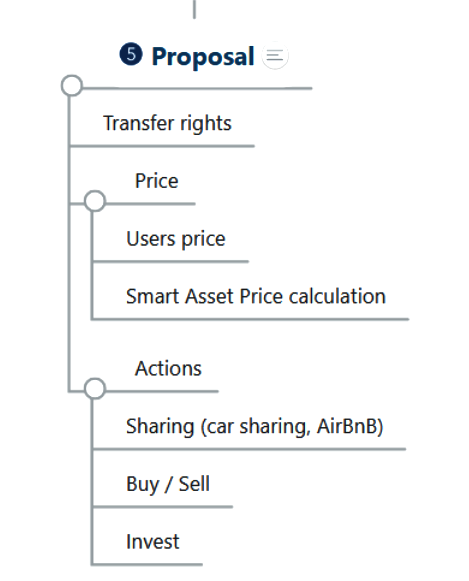
\includegraphics[width=0.4\textwidth]{proposal.png}
  \caption{SmartDeal Proposal Step}
  \label{fig:proposal}
\end{figure*}

The result of this step is the issuing of a token and formation of a bid for the Smart Asset Exchange.

\section{Technical solutions}

\subsection{IT Architecture Scheme}

IT architecture scheme is presented on Figure~\ref{fig:it-architecture}.

\begin{figure*}
  \centering
  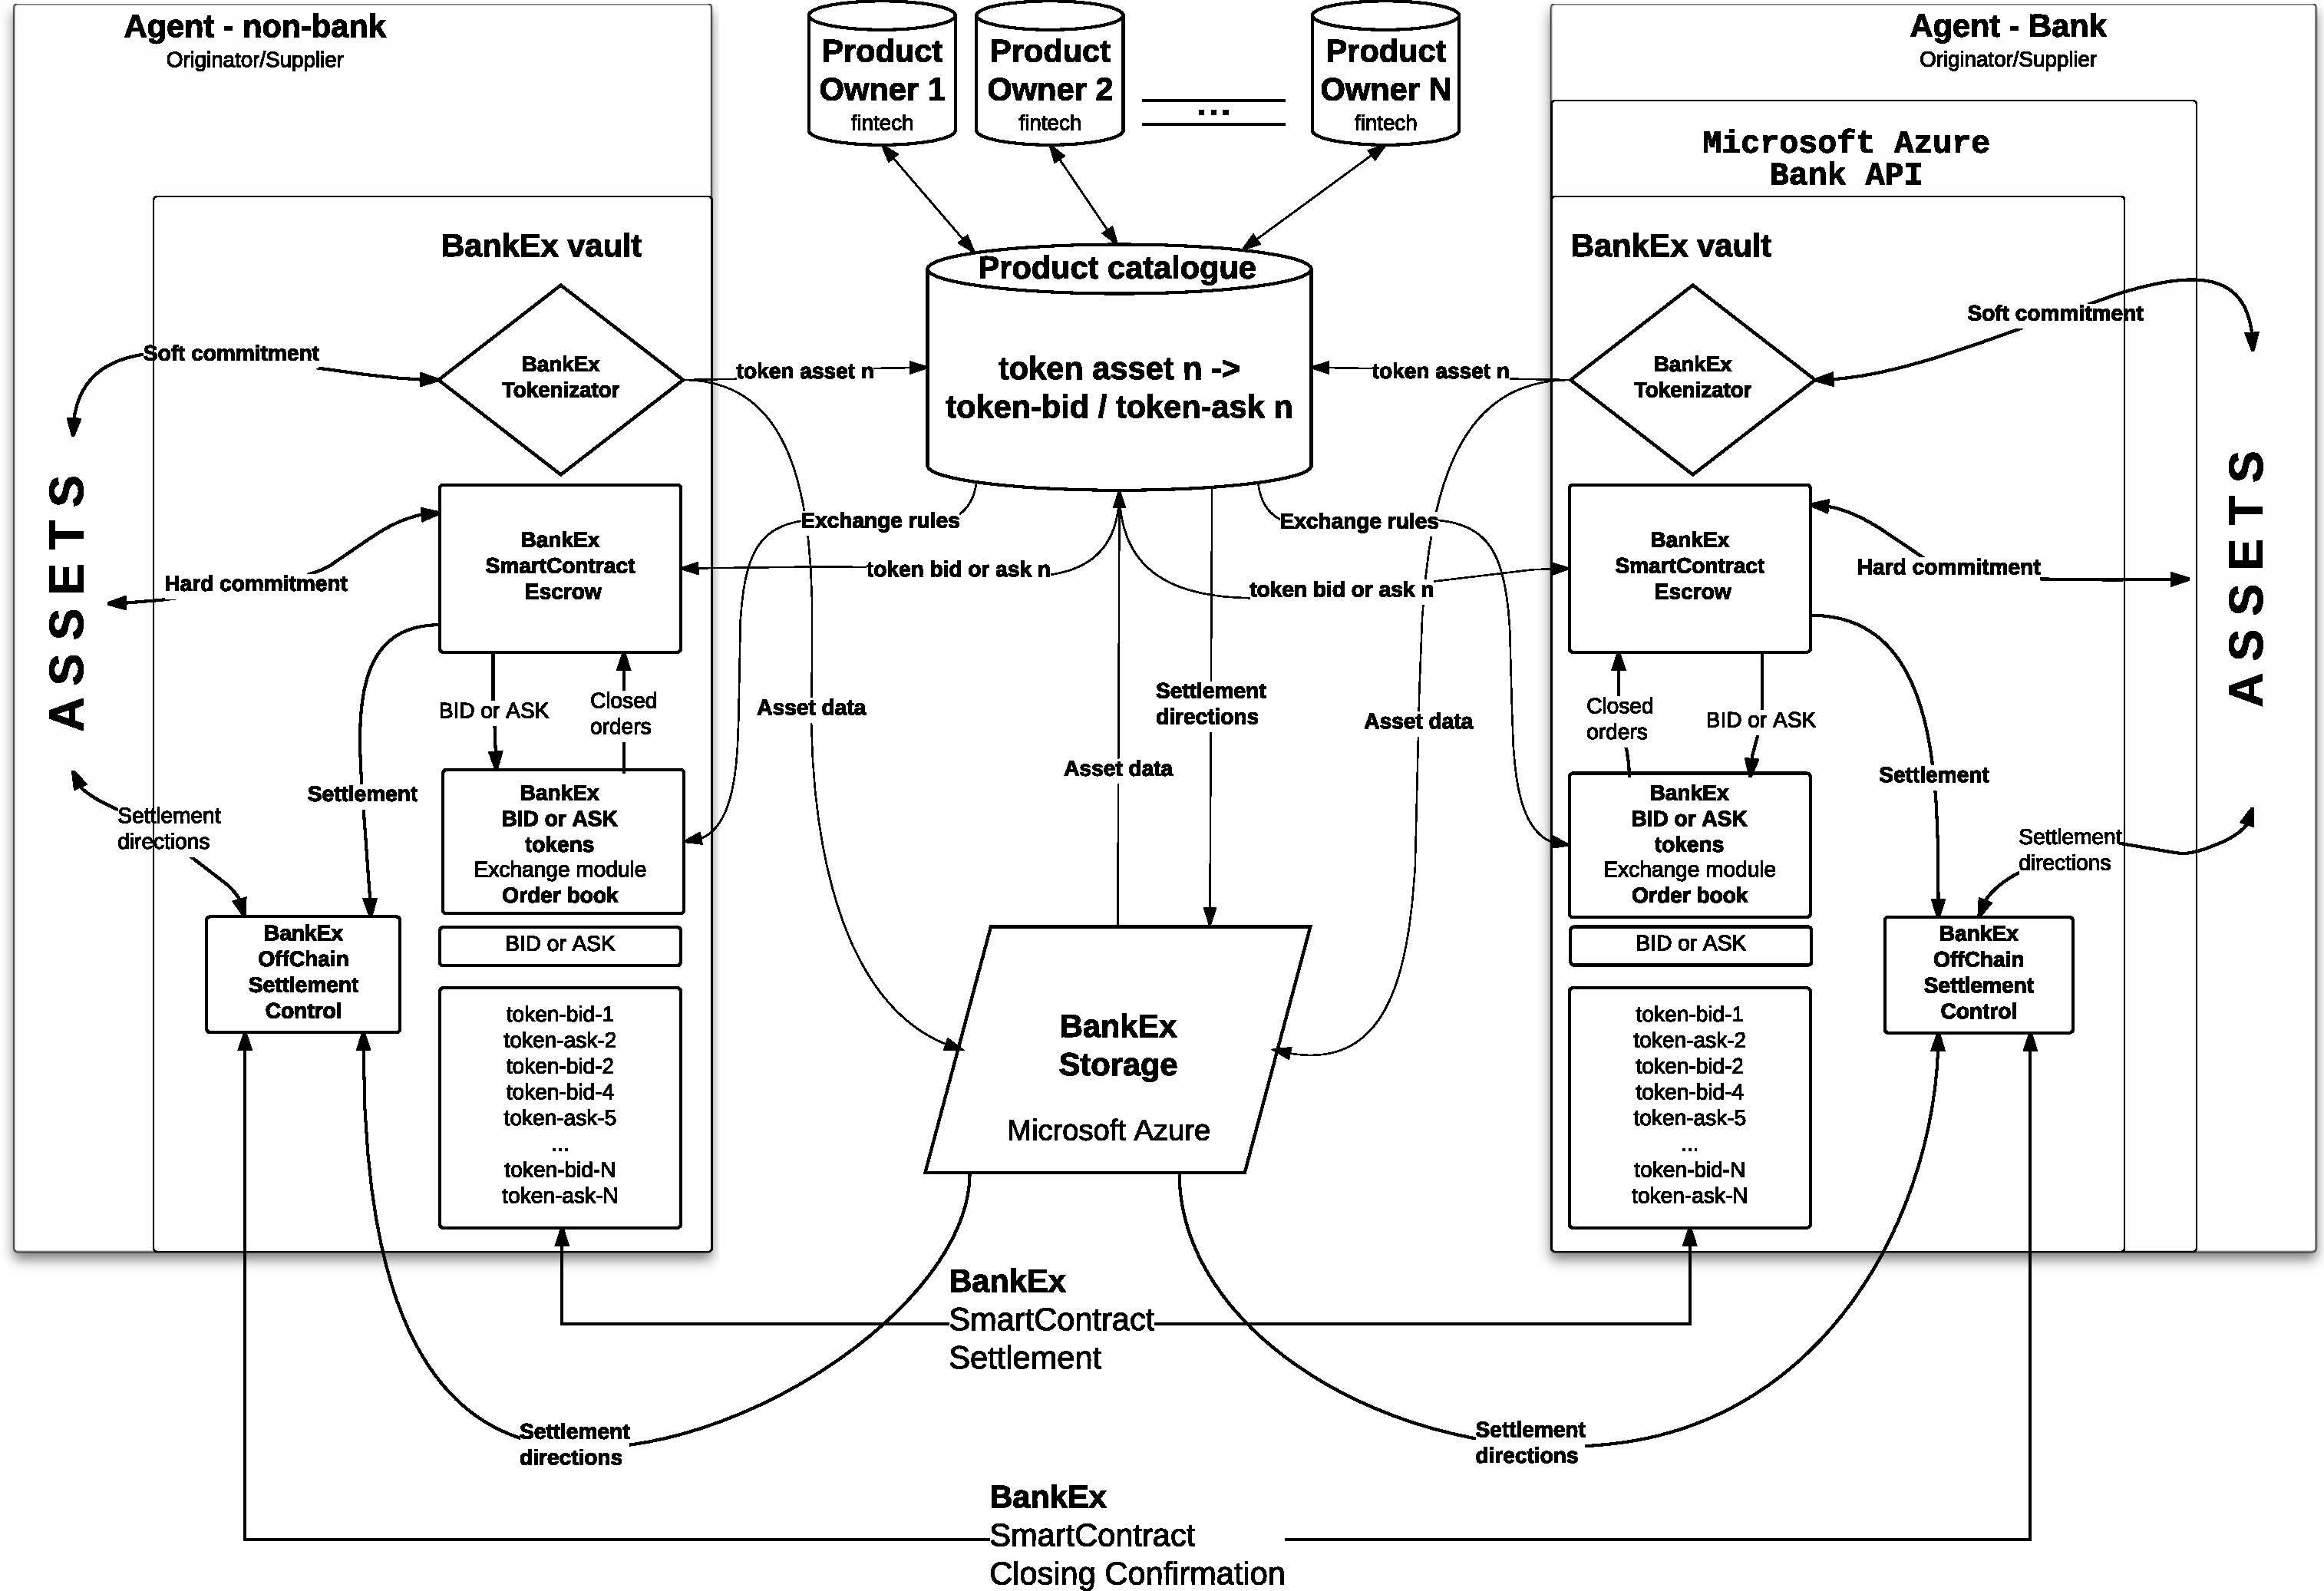
\includegraphics[width=\textwidth]{it-architecture.pdf}
  \caption{IT Architecture Scheme}
  \label{fig:it-architecture}
\end{figure*}

\subsection{Asset data compression for blockchain record}

\text{ }

\subsection{Role and system access matrix}

\text{ }

\subsection{Originator/Supplier interaction in the ecosystem architecture}

\text{ }

\subsection{Bank \& non-Bank Originator/Supplier}

\text{ }

\subsection{Use of Microsoft Azure Bank API}

\text{ }

\subsection{Large data volume hashing in the Microsoft Azure Storage}

\text{ }

\subsection{Soft and Hard Commitment assignment rules}

\text{ }

\subsection{Bid \& Ask records independence principle}

\text{ }

\subsection{Decentralized Order Book rules}

\text{ }

\subsection{Decentralized matching~--- pros and cons}

\text{ }

\subsection{Offchain Settelment Control}

\text{ }

\subsection{Settelment directions}

\text{ }

\subsection{Formula 1: saturation of request with data in a blockchain environment}

\text{ }

\subsection{Reasons for differentiation between order and bid for Smart Assets}

\text{ }

\subsection{Formula 2: solution for automated order merging and separation}

\text{ }

\subsection{Formula 3: filter cascade system in the Order Book}

\text{ }

\subsection{Formula 4: implementation of classical stock market trade rules in a blockchain environment}

\text{ }

\subsection{Study of speed parameters of matching for Smart Assets}

\text{ }

\subsection{Technological differences during Supplier tokenization}

\text{ }

\subsection{Transaction execution with decentralized storage}

\text{ }

\subsection{Work with order packages during contract initiation}

\text{ }

\subsection{Order of Escrow function in the transaction execution block}


\text{ }

\subsection{Smart Asset Core v.3}

Version 3 of Smart Asset Core is presented on Figure~\ref{fig:sa-core-v3}.

\begin{figure*}
  \centering
  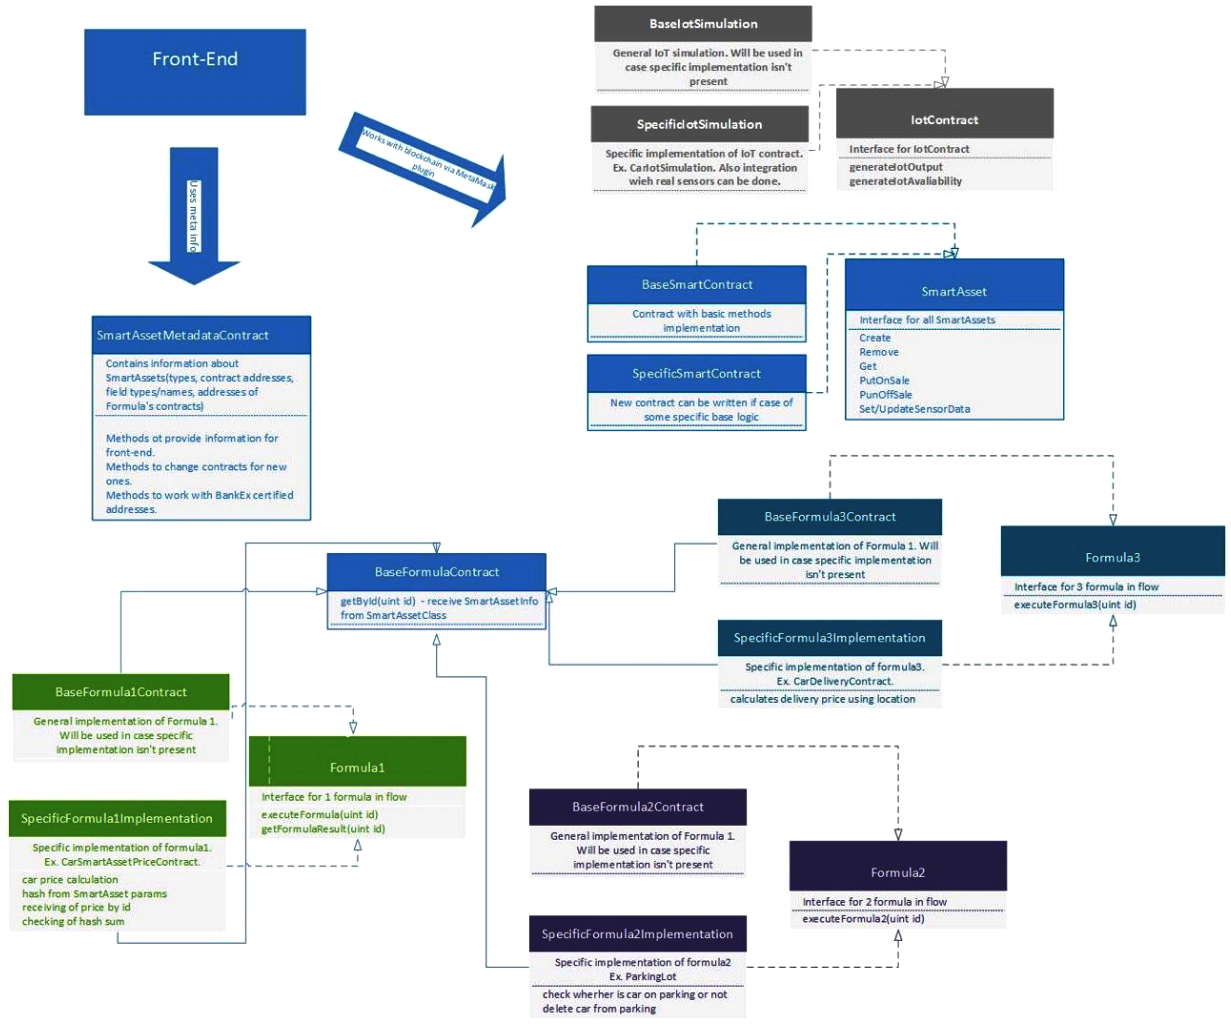
\includegraphics[width=\textwidth]{sa-core-v3.png}
  \caption{Smart-Asset Core, Version~3}
  \label{fig:sa-core-v3}
\end{figure*}

\subsection{Smart Asset Core v.4}

\text{ }

\subsection{\enquote{Plasma} protocol \& Proof-of-Asset Protocol}

A \enquote{Plasma} protocol was proposed recently, that is universal extension of any Turing-complete blockchain (such as Ethereum)  and allows creation of \enquote{daughter} blockchains that are governed by higher-level (\enquote{parent}) blockchain. These \enquote{daughter} chains can have different consensus rules, functionality (extensions to EMV, for example) and underlying base token. 

Such extension naturally fits Proof-of-Asset proposal with Bankex token (BKX) being an underlying currency used to pay for manipulations with asset records. If functional requirements for some types of assets or operations would impose a need of extended functionality, such type of assets can be moved to separate chain. These \enquote{daughter} chains can be viewed as side-chains for ease of understanding properties, but strongly governed and penalized by \enquote{parent} chain for any sign of misbehavior of fraud. Such approach and further extension of \enquote{daughter} - \enquote{parent} relation to the whole tree of chains would allow participants of Bankex protocol to effectively do transactions with minimal trust and be able to be minimally exposed to potential fraudulent actions of other participants, especially ones not even related to their current transaction, in contrast to traditional single level chain, where potential attack affects all users immediately (DAO hack, for example). 

\subsection{The most important features of Plasma protocol}

One of the most important features of Plasma protocol is an ability to extend EMV and add required functionality, that is now only possible by use of external oracles. One of such examples would be a development of \textit{JWT} (JSON Web token) like message exchange format with mandatory cryptographic signatures, that would allow some form of replayability and authentication of requests to external resources. Such exchange format and use case can be illustrated as following:
Over the lifetime of smart asset some data from external service (External API request)
Traditionally it’s solved by use of external oracle (such as oraclize.it), that performs a request on your behalf, provides some proof of authenticity (\textit{TLS Notary}) and performs a callback.
Such operation is expensive and requires few roundtrips. TLS Notary is not possible in modern versions of TLS protocol.

Our proposed approach would be to build a standard requests protocol that would start with pre-signed (by smart-contract itself or other way) payload, that can be used to perform a request to external resource at some timeframe and requiring a response to be signed by private key of external resource (with public key also known upfront). Also, standard would require that ANY request with such payload would return THE SAME response, so it would allow to perform distributed computing and easy verification for including information into the blockchain.

Another interesting extension would be possibility to perform \enquote{delayed calls}~--- requests to a smart asset functions that should be performed either at known date or regularly. For now such action would also require an external oracle, while such information can potentially be saved inside a blockchain, so every participant could trigger a function execution for an incentive in a form of fee (similar to the gas price).

At some point an extension of EMV can be required to facilitate new requirements or have backward compatibility with older systems. Such functionality can be RSA functions (for old systems), Schnorr signatures (can be extended already as convenience method) or post-quantum cryptography. We see a need in having a degree of backward compatibility to connect existing systems to blockchain.

But the most tedious questions to be solved for wider applications of blockchain, where computations are transparent, are, in our opinion, random number generation and homomorphic cryptography. First one is the cornerstone of cryptography in general and a way of obtaining a random number of appropriate quality will be a major breakthrough in a field. The latter is, for now, the only known possible way to achieve privacy and computation transparency at the same time. We think that extensive development and experimenting in this field should start as soon as possible, with choice of currently known candidates and implementing them in a \enquote{subchain} to which data can be transferred, manipulated and returned to the parent chain without disclosure of nature of underlying data.

\subsection{IoT Integration Scheme}

One of the necessary steps for IoT-enhanced assets is the procedure of integrating them with the IoT device control infrastructure. The procedure is shown on the Figure~\ref{fig:iot-user-story}.
There are four major layers of back-end applications involved:

\begin{figure*}
  \centering
  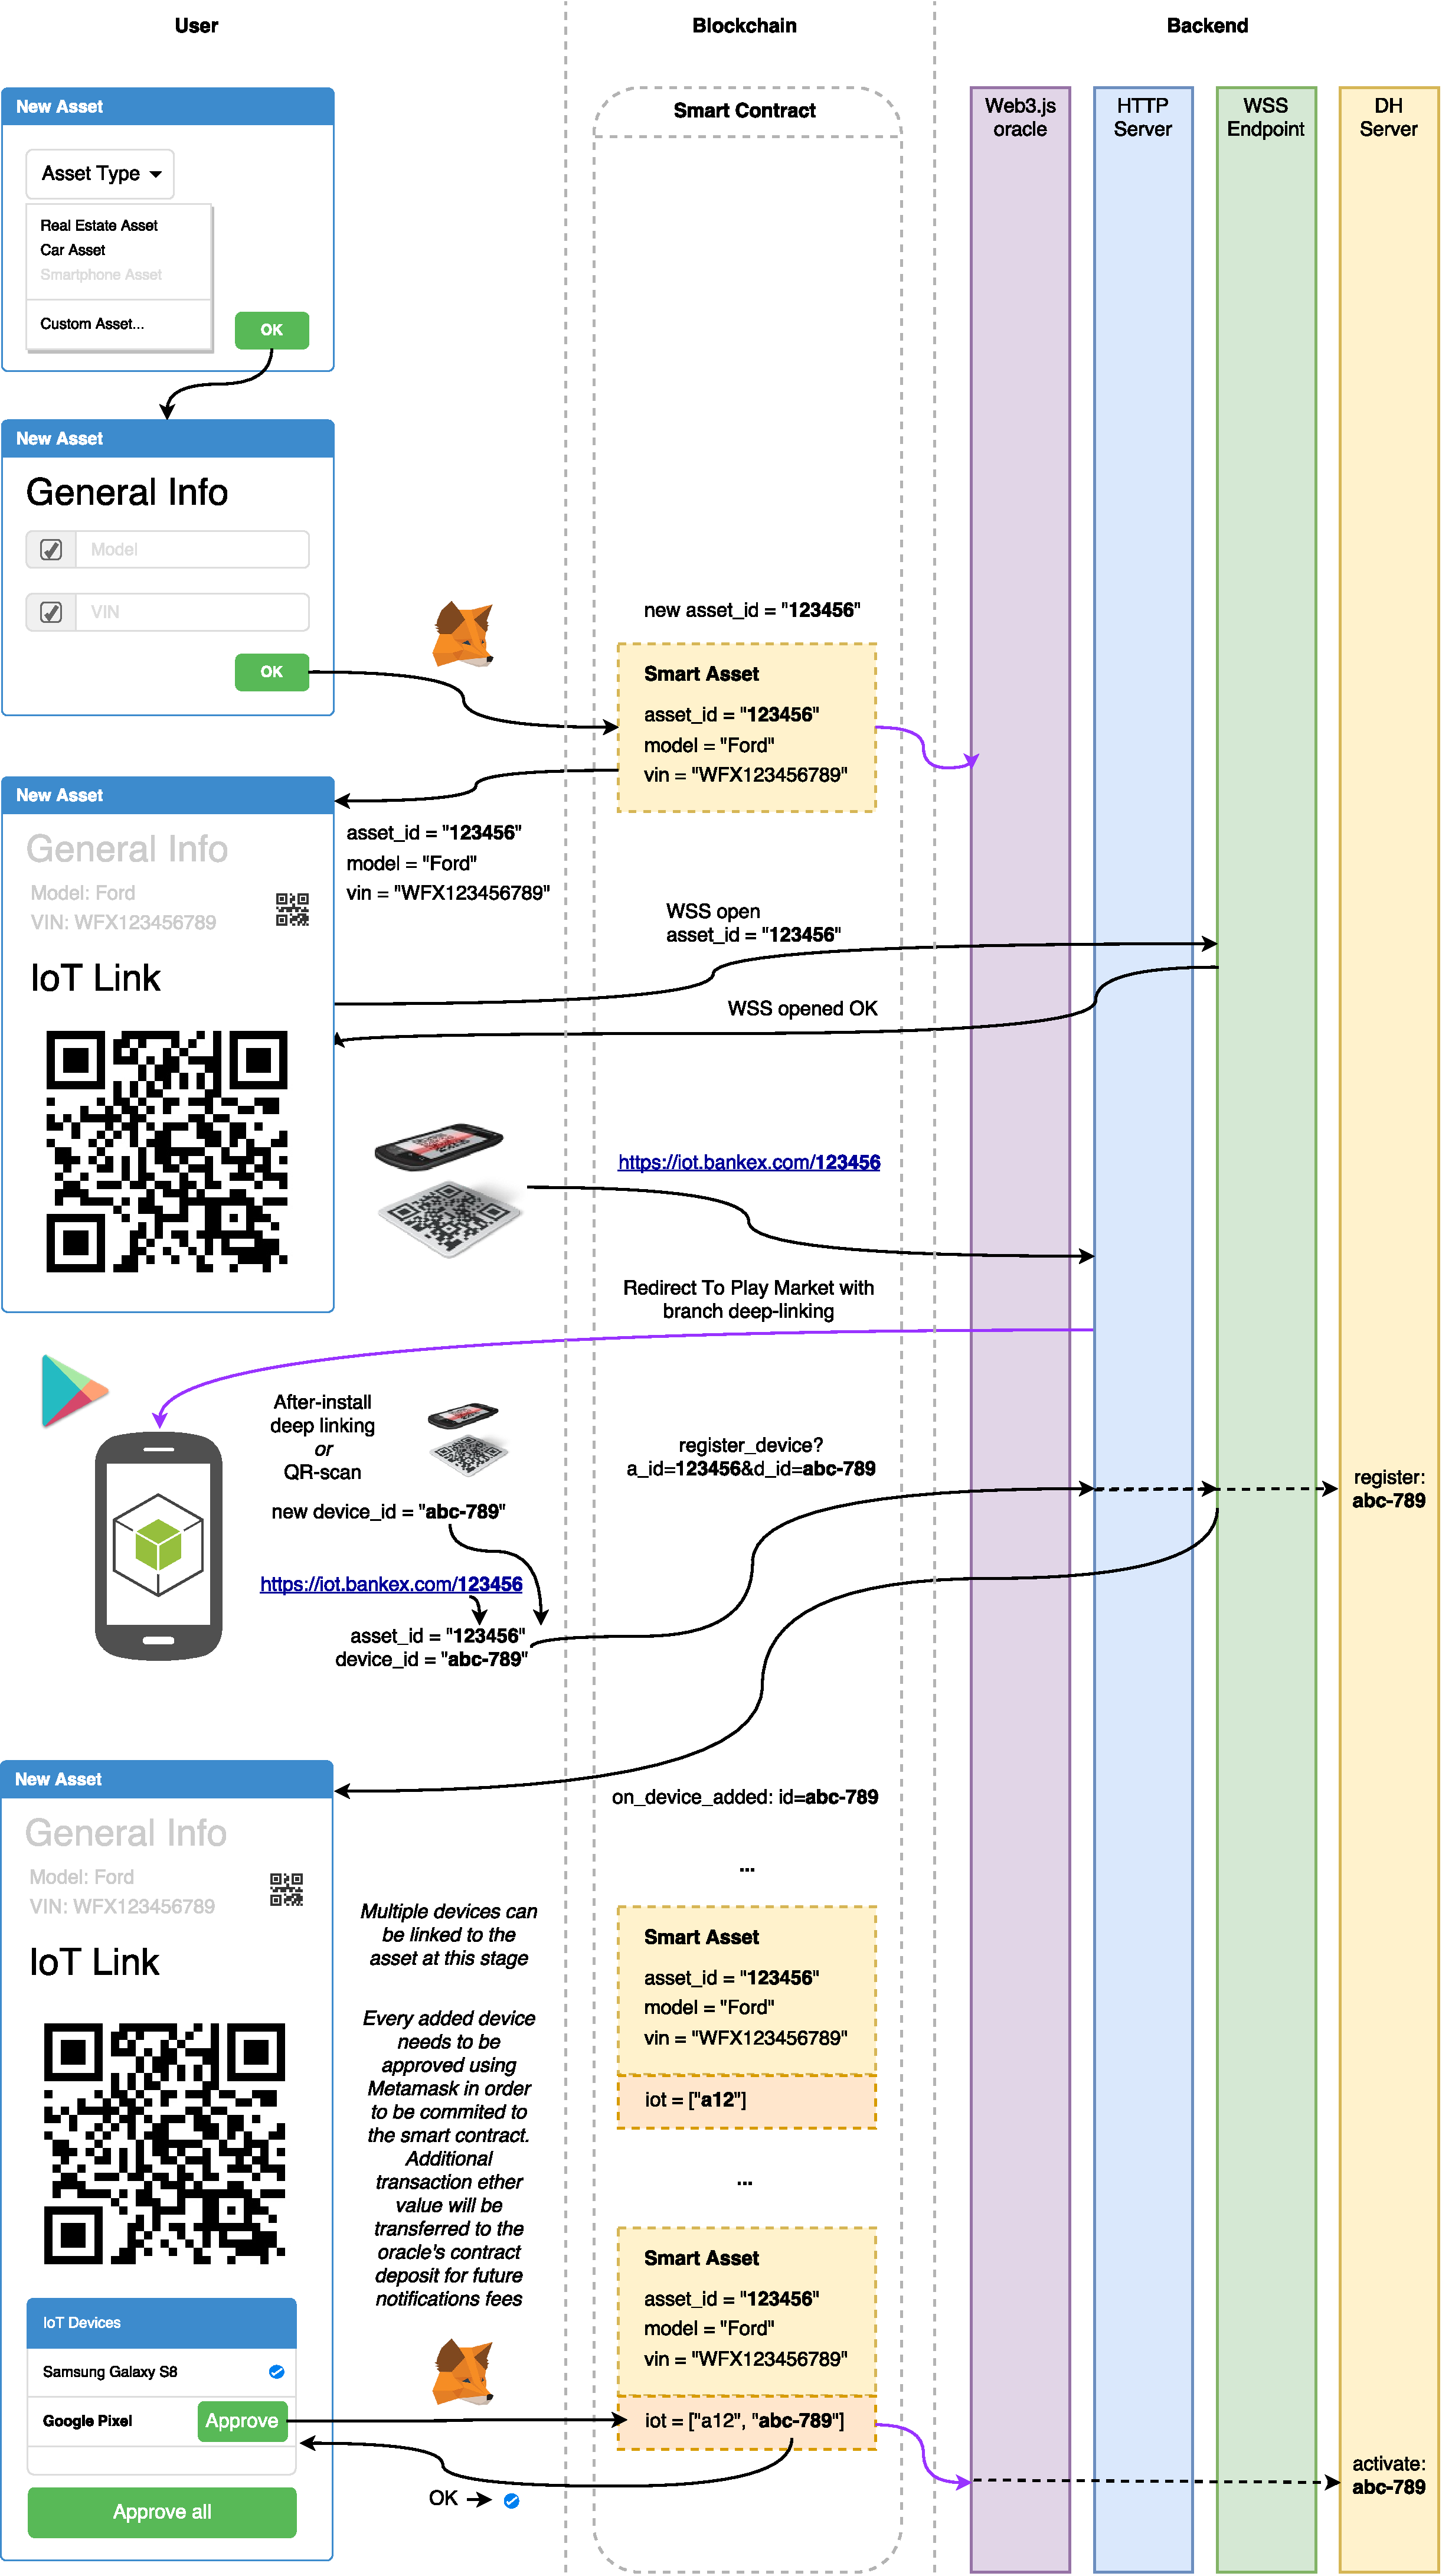
\includegraphics[width=0.75\textwidth]{iot-user-story.pdf}
  \caption{IoT--Asset Integration: the User Story}
  \label{fig:iot-user-story}
\end{figure*}

The backend consists of four primary server applications:

\begin{enumerate}
\item web3j-compatible connector to the Ethereum network node;
\item TLS-secured web server for serving HTTPS-requests for both API and frontend;
\item secured WebSocket server (\url{wss://});
\item DeviceHive\footnote{\url{https://devicehive.com/}} server for IoT device management.
\end{enumerate}

Let us describe the full process of integration in the case of a web-application (with a MetaMask extension installed) and the Android IoT App

\begin{enumerate}
\item The asset owner selects one of the types provided.
\item Initial data on the asset is filled in by its owner. After all the information is filled in, the user initiates the procedure of publishing the asset on a blockchain by using the contract function via MetaMask. On this stage we learn the newly created asset’s unique identification, which the client receives following a successful transaction.
\item After receiving the asset ID, the web interface moves on to the next step. The first thing that is required is a backend connection between the ongoing web-session and the ID of the newly created asset, which is done using a WebSocket connection. Until this step only the client and the blockchain are aware of the asset, and unless it is taken backend won’t be able to send events from the server, if they are linked to the current asset. A WebSocket connection solves this problem.
\item To connect the asset to IoT devices, the web page displays a specially generated QR-code, containing a link to the asset ID \url{http://iot.bankex.com/ASSET_ID}.
\item The user scans this code using the BANKEX IoT App. If it’s not installed, the code can alternatively be scanned by any QR-code scanner application, which is going to open the link in a browser, automatically redirecting the user to App Store or Play Market to download the application. Deep-linking support allows the application to be launched with additional parameters, including the asset ID, immediately after installation, which helps prevent scanning the same QR-code twice.
\item BANKEX IoT App is now ready to connect the asset ID to the ID of the device, which the application already knows at this point. In a simpler case, the BANKEX IoT App already supports the phone’s sensor identification, which requires no additional tools to demonstrate capabilities. External sensors can also be added using this application. 
\item The device contacts API, sending two key parameters: asset ID and device ID. This information is also shared with the DeviceHive, where the new data is automatically registered, as well as WebSocket to inform of the client’s newly added device. 
\item At this stage, the device ID is not yet added to the smart asset, although it is visible in the web client in the list of devices available to be added. To finish the integration, the user must confirm the device using the function in MetaMask. This transaction can charge additional Ether or BKX-tokens to credit the oracle’s IoT event execution expenses.
\end{enumerate}

\end{multicols}

\newpage
\appendix

\section{Terminology}
\begin{description}
\item[Blockchain]--- a cryptographically secured database containing the history of all transactions performed on the platform. It works the following way:
\begin{enumerate}
\item Transaction info is sent into the blockchain network
\item This transaction together with other transactions forms a block. Every block has its number and holds encrypted information about preceding blocks. 
\item The block is sent in to be checked by all members of the network
\item If there are no discrepancies, every member adds the new block to the chain of previous blocks and the transaction is executed. 
\end{enumerate}
\item[Node]--- a blockchain network participant storing information on past transactions (blockchain), checks information on new transactions for authenticity and is able to add in new transactions (adding blocks). All the nodes are connected to one another forming a single network. 
\item[A public blockchain] is a decentralized system where the information on transactions is stored and checked in many multiple locations. This kind of synchronization between millions of locations consumes large amounts of electric energy and is significantly more expensive than a private blockchain. The system also becomes slower. However, a public blockchain may prove preferable for industries where decentralization is necessary. 
\item[A private blockchain] is centralized, making it similar to traditional centralized systems, however it exceeds them in terms of efficiency and security.
\item[ICO (Initial Coin Offering)]--- a method of invitation to finance a campaign/project. Tokens/coins are issued that grant the right to receive a share/service/good now or in the future, or else they grant a percentage of future profits. After the start of sales, tokens can be resold to other investors. Trade is conducted on a blockchain. 
\item[Cryptocurrency]--- digital money without a physical analogue. It is supported by the complexity of its development~--- mining. Today we are able to identify \enquote{classics} such as Bitcoin or Litecoin, and newer currencies such as Ether, which act as platforms for the creation of new assets - tokens.
\item[Ethereum]--- the most popular platform for issuing of tokens and smart contracts. 
\item[Gas]--- a unit used to measure the price of calculations done on Ethereum. More difficult calculations are rewarded with higher amounts of Gas. This works the following way: the originator of a smart contract sets a price in gas. Miners, whose PCs handle the calculations, make the choice whether or not to perform these calculations. If the price offered is too low, then neither the calculations, nor, as a result, the contract will ever be concluded. 
\item[Smart-contract] a set of pre-programmed tasks that the program automatically carries out upon certain conditions being fulfilled, then forms a deal. That’s why it requires no trust between sides, nor a middleman: the contract has a strict logical structure and the computer executes it automatically. Smart-contracts allow for inclusion of a large number of conditions and states and for a correlation between their every possible combination and various outcomes. 
\item[Ditigal tokens]--- croptygraphic assets issued using specialized blockchain platforms. An analogue would be a record in a register. A token has an address and may also contain a smart-contract that defines its function and also acts as a separate execution mechanism. 
\item[Tokenization]--- the process of transforming rights into a digital token, which is then traded on a blockchain with low transactional costs. Tokenization is an analogue of securitization on a blockchain. 
\item[Smart Asset]--- an asset that has gone through tokenization using the BANKEX Proof-of-Asset Protocol. 
\item[ISAO (Initial Smart Asset Offering)]--- a method of fixing businesses (farms, stores, manufacturing plants) using tokenization of their assets based on the BANKEX PoA protocol. 
\item[Product instance]--- an iteration of a fintech-product owned by a BANKEX product provider. For instance a product provider can customize his product for various regions, thus creating a product instance for each country. 
\item[Blockchain-agnostic protocol]--- an application level protocol that does not depend on the exact blockchain-technology utilized and can be implemented on any existing open source blockchain. 
\end{description}

\printbibliography

\end{document}
